\documentclass[11pt]{article}
\usepackage[utf8]{inputenc}
\usepackage[T1]{fontenc}
\usepackage{amsmath,amssymb,amsfonts}
\usepackage[version=4]{mhchem}
\usepackage{graphicx}
\usepackage{booktabs}
\usepackage{siunitx}
\usepackage[margin=1in]{geometry}
\usepackage[hidelinks]{hyperref}
\usepackage{xr-hyper}
\externaldocument[][nocite]{SI}[SI.pdf]
\usepackage[numbers,sort&compress]{natbib}
\usepackage{xcolor}
\usepackage{authblk}
\usepackage{caption}
\usepackage{float}
\captionsetup{font=small,labelfont=bf}
\sisetup{detect-all}
\DeclareSIUnit{\Molar}{M}
\newcommand{\ci}{c_{\mathrm{I^-}}}
\newcommand{\cf}{c_{\mathrm{I_2}}^{\,\mathrm{f}}}
\newcommand{\csat}{c_{\mathrm{sat}}}
\newcommand{\epss}{\varepsilon_{\mathrm{s}}}
\newcommand{\epsl}{\varepsilon}
\newcommand{\iapp}{i_{\mathrm{app}}}
\newcommand{\Deff}{D_{\mathrm{eff}}}
\newcommand{\thetaeff}{\theta_{\mathrm{eff}}}
\newcommand{\thetacal}{\theta_{\mathrm{cal}}}
\newcommand{\thetaisland}{\theta_{\mathrm{island}}}
\newcommand{\Qfcal}{Q_{\mathrm{f,cal}}}
\newcommand{\mAcm}{\si{mA.cm^{-2}}}
\newcommand{\mAhcm}{\si{mAh.cm^{-2}}}

\title{\bfseries A zinc--iodine flow-battery positive-electrode model coupling
solid-iodine deposition and accessibility loss}

% --- Authors and affiliation: fill in with advisor ---
% \author[1]{Given Name}
% \affil[1]{Affiliation, City, Country}
\author{~}
\date{}

\begin{document}
\maketitle

\begin{abstract}
\noindent
In zinc--iodine flow batteries (ZIFBs), the positive carbon-felt electrode couples soluble-iodine
speciation, native-iodine deposition and progressive loss of electrochemically accessible area. We develop
a calibrated multiscale positive-electrode scaffold that distinguishes free-\ce{I2} saturation, retained
solid-iodine inventory and functional accessibility. In the registered production branch at
\SI{40}{mA.cm^{-2}} and in the representative \SI{1}{M}~\ce{ZnI2}$+$\SI{4}{M}~\ce{NH4Br}
electrolyte, the model reaches its positive-electrode-averaged $S_{\mathrm{base}}=1$ marker at
$Q_{\mathrm s}=\SI{83.0}{mAh.cm^{-2}}$ and the voltage-calibrated half-accessibility marker at
$\Qfcal=\SI{99.6}{mAh.cm^{-2}}$; smooth relative permeability remains $0.956$ at
\SI{120}{mAh.cm^{-2}}. Lower-scale calculations constrain placement, transport and physical closure families
rather than fixing calibrated accessibility. In fresh matched
true-mesh solves, replacing only the production accessibility relation with the dense physical-island relation
changes $Q_{\mathrm s}$ by only \SI{0.002}{mAh.cm^{-2}}, but changes the endpoint accessibility loss from
$0.990$ to $0.309$ and the voltage from \SI{1.728}{V} to \SI{1.440}{V} ($-\SI{288.2}{mV}$); the
physical-island case does not
reach half accessibility by \SI{120}{mAh.cm^{-2}}. This divergence shows that accessibility feedback changes
the solid-inventory and voltage trajectories, while voltage alone does not identify the deposit morphology.
Existing single-cell composition, rate and thickness data provide protocol-bounded context, with \ce{NH4Br}
serving only as a representative supporting electrolyte. The framework separates free-iodine saturation,
native-solid deposition and closure-dependent accessibility loss, and identifies the transport and morphology
parameters that move the modeled positive-electrode operating window.
\end{abstract}

\vspace{0.5em}\noindent\textbf{Keywords:} zinc--iodine flow battery; positive electrode; iodine
super-saturation; accessibility loss; porous-electrode model; operating boundary; multiscale
modeling

\section{Introduction}
Zinc--iodine flow batteries (ZIFBs) are an attractive chemistry for low-cost, safe aqueous grid storage: they
pair an abundant, high-potential iodide/iodine catholyte with a zinc anode, decouple power from energy, and
reach high theoretical capacity, with recent cells pushing toward practical high areal loadings
\citep{Li2015,Xie2018,Weng2017,Wen2025,Fan2024,Huang2025,WuLoading2025}. Realizing that promise at high
loading and high current, however, is limited less by the redox couples themselves than by what the charged
phases do inside the porous electrodes.

A practical ZIFB has several coupled failure channels. On the negative side, non-uniform zinc plating forms
dendrites and a compact zinc layer near the electrode--membrane interface that starves the porous
felt of ions and can perforate the separator \citep{Richtr2026,ZnBr_CurrentDist2024,Guo2025}. In the
electrolyte, dissolved polyiodide can shuttle across the membrane and self-discharge the cell
\citep{LiuMembrane2025,Wei2025,XuZnBr2024}. On the positive side, the iodine redox must run through a poorly
soluble neutral intermediate: charging oxidizes iodide to \ce{I2} ($2\,\ce{I^-}\rightarrow\ce{I2}+2e^-$),
which iodide immediately binds into soluble triiodide
($\ce{I^-}+\ce{I2}\rightleftharpoons\ce{I3^-}$, $K\approx698~\mathrm{M^{-1}}$ \citep{Palmer1984,Wen2025}).
Most of the oxidized iodine is thus \emph{hidden} in a soluble complex, so precipitation is governed not by the
total oxidized inventory but by the small \emph{free} \ce{I2} monomer left over: once that free monomer outruns
the buffer it can precipitate as native \ce{I2}(s). Independent electrochemical and confined-host studies
resolve or retain solid iodine under their own electrode conditions \citep{Fitzek2023,SolidI2_NatCommun2020};
they do not establish the deposit geometry in the present carbon felt.

The negative-side and shuttle channels have received sustained mechanistic attention, but the positive iodine
electrode is less resolved. Its failure is subtler than a solubility limit. Retained \ce{I2}(s) is not,
by itself, the failure: a solid can sit in the felt without occluding the percolating reaction and transport
network; it becomes limiting only once its morphology overlaps the active area and the ion/mass-transfer
paths. Both sides of that distinction have host-specific precedents. In-situ optical microscopy in a
distinct dual-plating, static graphite-felt iodine chemistry resolves a continuous \ce{I2} film during charge
and discrete residual particles after discharge \citep{LiDualPlate2025}. A nanoconfined activated-carbon
platform reports at least about $30\%$ iodine pore filling while retaining high coulombic efficiency and
cycling stability \citep{SolidI2_NatCommun2020}; this is a host-bounded counterexample, not a felt threshold.
A dense iodine film can raise positive-electrode charge-transfer resistance
roughly ninefold \citep{Jang2021}. Dissolution measurements also show that solvent environment changes the
solid-iodine clearance scale and high-rate response \citep{Zhao2022}. The unresolved modeling question is
therefore not only the \emph{appearance} of iodine but the state relation by which retained inventory becomes
associated with loss of electrochemically accessible area. Continuum porous-electrode theory is well established for this kind of
question---from the classical framework of Newman and co-workers \citep{Newman1962} to modern
tertiary-current-distribution solvers for flow cells \citep{Tichter2020,Chakrabarti2020,AparicioMauricio2023},
and to reduced-order models of solid-product passivation in \ce{Li}--\ce{S} and related electrodes
\citep{LiS_ROM_JES2025}---but none of these resolves, for the iodine positive electrode, the specific map from
retained native \ce{I2}(s) inventory to \emph{functional} accessibility and transport loss. For that
transition, an auditable, conditional electrode-resolved scaffold that separates an averaged saturation
marker from morphology-dependent accessibility loss remains missing.

The supporting electrolyte here is \ce{NH4Br}. It is treated as a representative formulation context rather
than the paper's protagonist: the modeled positive-electrode branch is \ce{I2}/\ce{I^-}, not bromide oxidation.
Composition-dependent speciation and transport require separate measurements and are therefore discussed
descriptively (\S\ref{sec:compmodule}, \S\ref{sec:chemaxis}).

Here we build a calibrated iodine-state scaffold for the ZIFB positive electrode
(Fig.~\ref{fig:concept}). The continuum model supplies spatial fields of free-iodine stress and retained
solid fraction. DFT supplies a relative placement tendency at oxygenated carbon sites, not an absolute
nucleation density; molecular dynamics supplies a bounded bulk-electrolyte carrier-diffusivity prior; the
single-fibre calculations define isolated-island accessibility families; and the pore-network calculations
bound the smooth bulk-permeability response. The effective accessibility magnitude used by the production
continuum branch is calibrated to the voltage response and is therefore kept distinct from the physical
isolated-island closure (Fig.~\ref{fig:provenance}). We organize the resulting charge trajectory as a state
clock in areal capacity $Q$ and project it into a positive-electrode $J$--$Q$ map. Published iodine-dissolution
measurements provide condition-specific external kinetic scales through $i^{*}=2Fk$ \citep{Zhao2022}; they do
not measure a universal current ceiling for the present electrolyte. The model resolves one galvanostatic
charge and does not establish cycle-to-cycle reset, discharge recovery or a unique deposit morphology.
Existing compression, composition and rate data are reported with their source-specific roles as descriptive
external-consistency evidence; they do not independently validate the production thresholds.

\begin{figure}[tbp]\centering
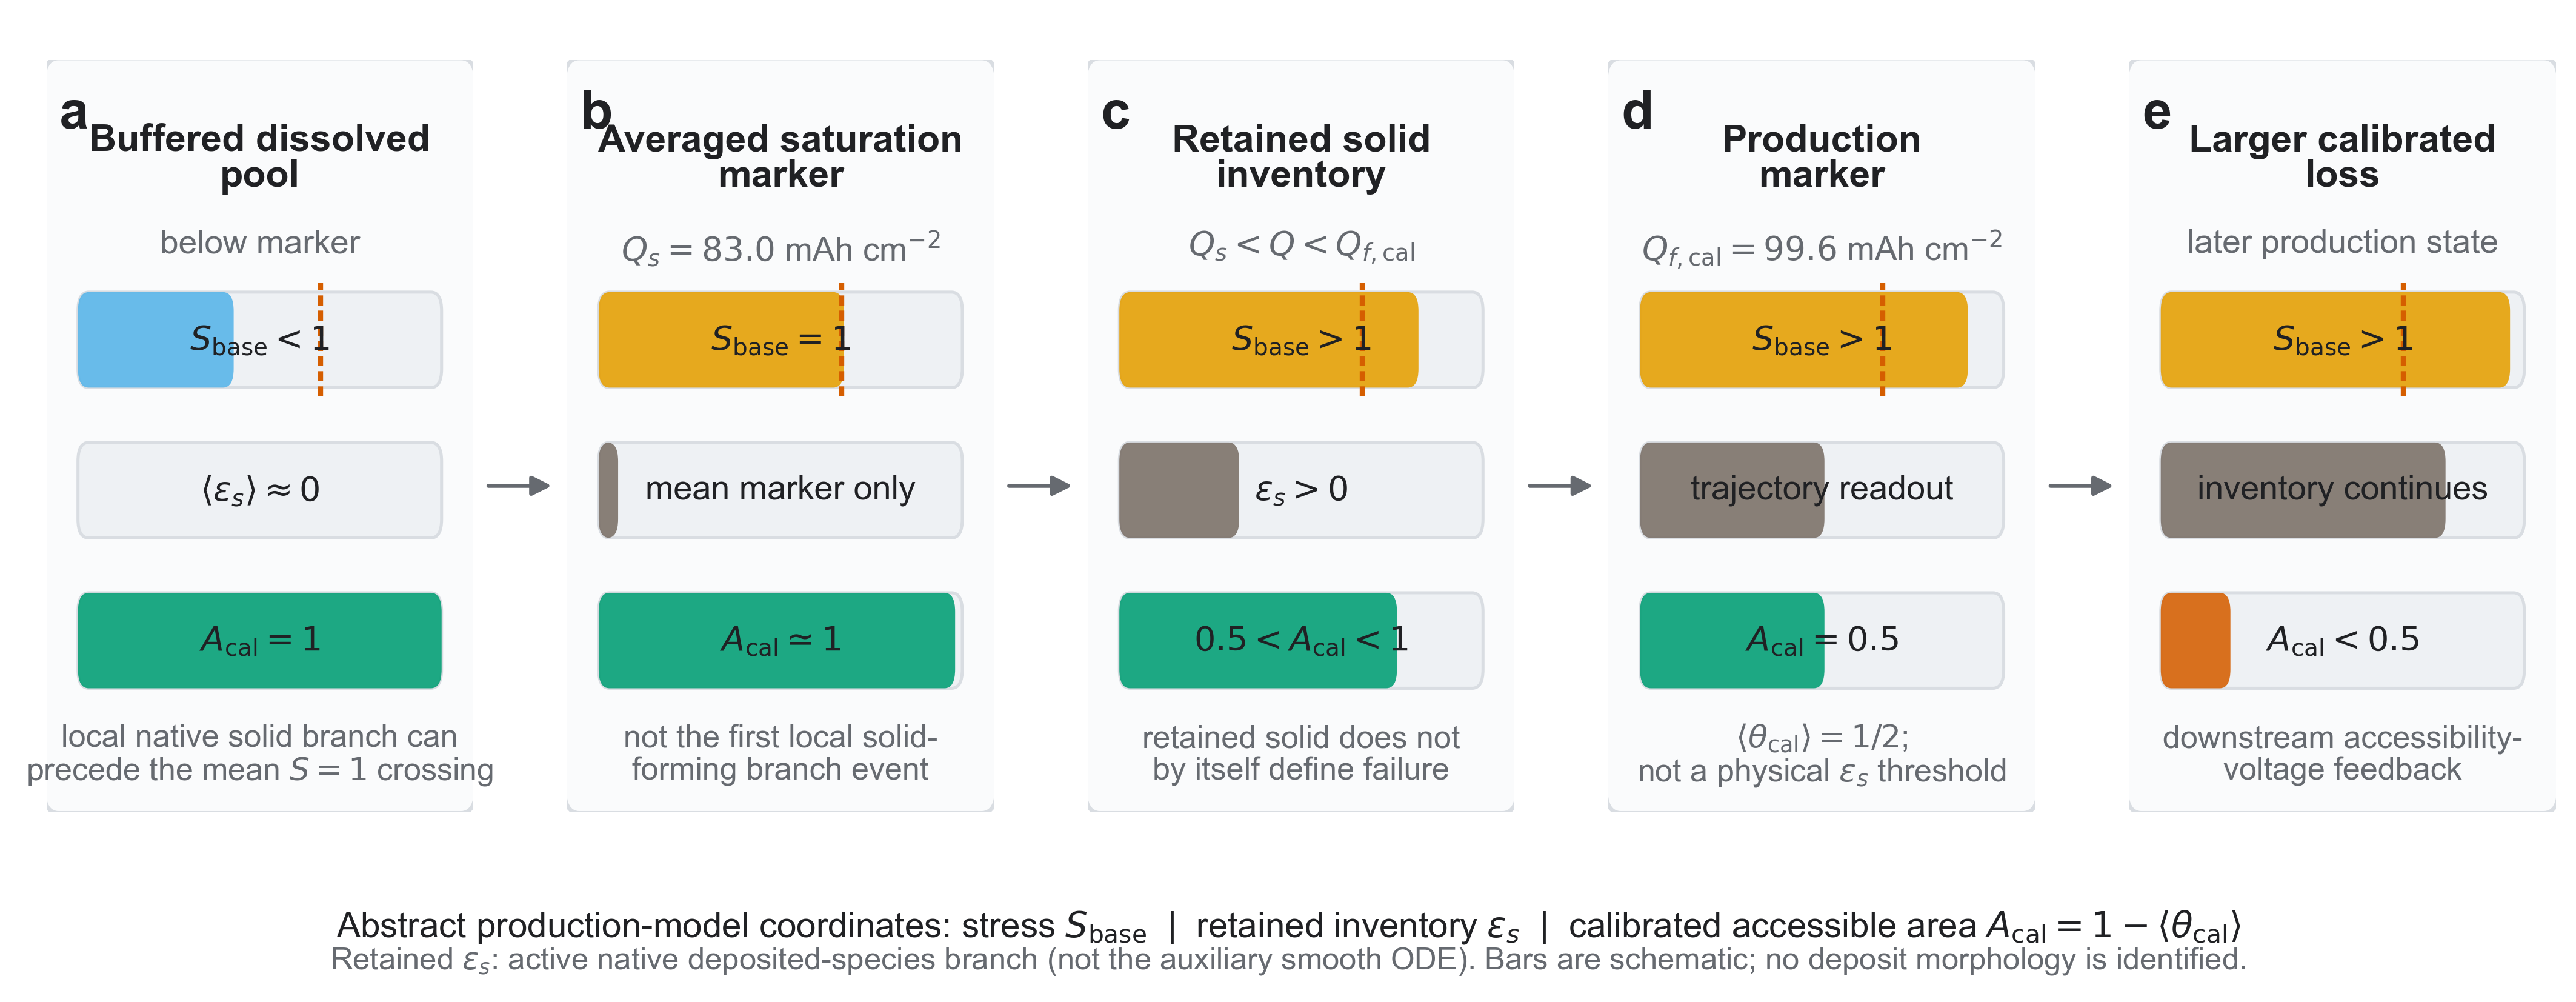
\includegraphics[width=\textwidth]{figures/Fig_R581_concept_state_progression.pdf}
\caption{\textbf{Conceptual iodine-state progression in the ZIFB positive electrode.}
(a)~Before the registered averaged marker, the mean oxidized-iodine inventory remains dominated by the
dissolved, buffered pool; local native-solid-path activation can precede that mean crossing.
(b)~The production model defines its registered averaged-saturation marker by $S_{\mathrm{base}}=1$.
(c)~Beyond the registered saturation marker, retained \ce{I2}(s) can accumulate while substantial reaction
area remains accessible.
(d)~The production branch defines its functional marker by
$\langle\thetacal\rangle=\tfrac12$, not by the physical-island or film-percolation solid fraction.
(e)~Larger effective accessibility loss is a downstream modeled state. At the registered baseline,
$Q_{\mathrm s}=\SI{83.0}{mAh.cm^{-2}}$ and $\Qfcal=\SI{99.6}{mAh.cm^{-2}}$. The artwork defines model
states; it is not an image of the deposit and does not identify a continuous film or local pore-throat
blockage. The scale-to-variable evidence types are summarized in Fig.~\ref{fig:provenance}.}
\label{fig:concept}
\end{figure}

Solid reaction products passivate or disconnect the active surface in other aqueous and
condensed electrodes, from \ce{ZnO} to \ce{Li2S} and \ce{MnO2} \citep{ZnO_EEM2024,Li2S_EcoMat2024,YangZnMn2026};
the iodine case differs mainly in lacking such a porous-electrode map, and it is that map this work supplies.

\section{Model framework and reduced iodine-state theory}
\label{sec:theory}
The positive-electrode scaffold follows one state chain: free-\ce{I2} super-saturation
$S_{\mathrm{base}}$ drives retained solid fraction $\epss$, and an accessibility closure maps $\epss$ to
loss of electrochemically reachable area. The registered production branch defines the averaged-saturation
marker $Q_{\mathrm s}$ by $S_{\mathrm{base}}=1$ and a calibrated half-accessibility marker $\Qfcal$ by
$\langle\thetacal\rangle=\tfrac12$. Physical isolated-island and film-percolation thresholds are separate
comparators. This section defines the state chain and its closure-conditioned operating boundary; the continuum
implementation is deferred to \S\ref{sec:multiscale}. Charging oxidizes iodide,
$2\,\ce{I^-}\rightarrow\ce{I2}+2e^-$, but a complexation buffer
$\beta = 1 + K_{\mathrm I}c_{\ce{I^-}} + K_{\mathrm{Br}}c_{\ce{Br^-}}$ holds the \emph{free} \ce{I2}
concentration $\cf = c_{\mathrm{I_2,tot}}/\beta$ below the effective saturation $\csat^{\mathrm{eff}}$. The super-saturation
$S=\cf/\csat^{\mathrm{eff}}$, not the total oxidized inventory, therefore defines the model's operational
saturation coordinate. Local regions can cross $S=1$ and activate the native-solid branch before the
electrode average reaches unity, so $Q_{\mathrm s}$ is not the first local solid. Three state variables then carry
the model: $S_{\mathrm{base}}$, $\epss$ and a named accessibility loss---$\thetacal$ for production or
$\thetaisland$ for the physical-island branch. The production interval
$\Delta Q_{\mathrm{cal}}=\Qfcal-Q_{\mathrm s}$ is therefore a closure-conditioned state-clock output
(Fig.~\ref{fig:concept}b--d). The accessible fraction is $A_{\mathrm{bare}}=1-\theta$; we avoid using
``coverage'' as a morphology label because voltage does not identify the deposit geometry.
The free-\ce{I2} super-saturation
that produces the solid is itself a \emph{mass-transfer} stress, set by the oxidized-carrier diffusivity, the
boundary layer, and the accommodation chemistry. A slower-diffusing electrolyte therefore moves the
boundary through transport rather than through accessibility alone; viscosity acts separately through the
Darcy-pressure channel unless it also changes diffusivity. Because the generation load rises with current density
$J$ and the inventory with capacity $Q$, $S$ is a function of the operating point $(J,Q)$. The saturation and
calibrated-accessibility markers become two curves in the $J$--$Q$ plane. Published dissolution measurements
provide the condition-specific scale $i^{*}=2Fk$, rather than a universal ceiling for this electrolyte. The rest of this
section makes that picture quantitative, building in turn the reduced one-carrier scaffold (\S\ref{sec:gov}),
the closures that fix its coefficients (\S\ref{sec:closures}), the super-saturation stress (\S\ref{sec:nondim}),
and the resulting $J$--$Q$ boundary with its production markers and external kinetic scale
(\S\ref{sec:jq}--\ref{sec:diss}), before separating supporting-electrolyte context (\S\ref{sec:compmodule}).
The explicit continuum governing balances and their assumptions are deferred
to the implementation (\S\ref{sec:backbone}); symbols are collected in Table~\ref{tab:notation}.

\begin{table}[t]\centering\small
\caption{Principal symbols and baseline values (bulk electrolyte \SI{1}{M}~\ce{ZnI2} $+$ \SI{4}{M}~\ce{NH4Br},
i.e.\ bulk $c_{\ce{I^-}}=\SI{2}{M}$ and $c_{\ce{Br^-}}=\SI{4}{M}$; $i_{\mathrm{app}}=\SI{400}{\ampere\per\meter\squared}$,
$T=\SI{293.15}{\kelvin}$ in the registered continuum solve). The buffer $\beta$ (and hence $S_{\mathrm{base}}$) is evaluated at the
\emph{current-on surface-effective} iodide, not the bulk value; this boundary-layer reduction is derived in
\S\ref{sec:gov}. Reused letters are kept distinct: the dissolution constant $k$ ($i^{*}=2Fk$), the
accessibility prefactor $k_{\mathrm{geo}}$, and the complexation constants $K_{\mathrm I},K_{\mathrm{Br}}$ are
different quantities.}
\label{tab:notation}
\begin{tabular}{@{}l p{0.46\linewidth} p{0.32\linewidth}@{}}
\toprule
symbol & meaning & value / units \\
\midrule
$n,F$ & electrons per \ce{I2}; Faraday & $2$; \SI{96485}{\coulomb\per\mol} \\
$c_{\mathrm{I_2,tot}},\cf$ & total / free dissolved \ce{I2} & \si{\mol\per\meter\cubed} \\
$\csat$ & \ce{I2} saturation reference & \SI{1.33}{\mol\per\meter\cubed} \\
$\beta$ & complexation buffer $1+K_{\mathrm I}\ci+K_{\mathrm{Br}}c_{\mathrm{Br}}$ & $554$--$1263$ (surface) \\
$D_0,\Deff$ & free-solution / Bruggeman oxidized-carrier diffusivity (lumped \ce{I3^-}/\ce{I2Br^-}; the neutral-\ce{I2} prior is $0.6\times10^{-9}$, SI) & \SI{0.5e-9}{}; $D_0\epsl^{1.5}$ \si{\meter\squared\per\second} \\
$\delta$ & Nernst-layer thickness & \SI{25e-6}{\meter} \\
$\epsl,\epss$ & pore-liquid / solid-\ce{I2} fraction & $\epsl=\varepsilon_0-\epss$ \\
$V_m$ & molar volume of \ce{I2}(s) & \SI{5.15e-5}{\meter\cubed\per\mol} \\
$Q$ & areal capacity (charge clock) & \si{\milli\ampere\hour\per\centi\meter\squared} ($=\SI{3.6e4}{\coulomb\per\meter\squared}$) \\
$S$ & super-saturation stress $\cf/\csat^{\mathrm{eff}}$ & dimensionless \\
$S_{\mathrm{base}}$ & within-cycle baseline stress & $\gamma_{\mathrm{salt}}(\Pi_{\mathrm{inv}}+\Pi_{\mathrm{gen}})/\beta_{\mathrm{intra}}$ \\
$\thetacal$ & production voltage-calibrated accessibility loss &
$\Qfcal:\langle\thetacal\rangle=\tfrac12$ \\
$\thetaisland$ & physical isolated-island accessibility loss &
$1-\exp(-35.4\varepsilon_{\mathrm{s,reg}}^{0.6222})$ \\
$A_{\mathrm{bare}}$ & accessible carbon fraction in the active closure & $1-\theta$ \\
$N_{\mathrm{I_2}}$ & dynamic dimensionless state in the production accessibility relation & solved state \\
$N$ & swept areal-density prior in the physical single-fibre family & \si{\per\meter\squared} \\
$35.4,\ 0.6222$ & fitted dense-island coefficient and exponent (Eq.~\ref{eq:thetaclosure}) & dimensionless \\
$\varepsilon_{\mathrm{s,cal,traj}}^*$ & mean production solid fraction at $\Qfcal$ & $1.18572\times10^{-4}$ \\
$\varepsilon_{\mathrm{s,island},1/2}$ & dense-island half-accessibility fraction & $1.7973\times10^{-3}$ \\
$\varepsilon_{\mathrm{s,film\text{-}perc}}^*$ & geometric connected-film/percolation marker & $2.2324\times10^{-3}$ \\
$\phi_{\mathrm{ppt}}$ & reduced solid-formation efficiency per unit overshoot $(S-1)_+$ & dimensionless; closure-cond. \\
$i^{*}=2Fk$ & condition-labelled dissolution-derived current scale & \si{\ampere\per\meter\squared} \\
\bottomrule
\end{tabular}
\end{table}

\subsection{State variables and the reduced scaffold}
\label{sec:gov}
We write the reduced criterion along the through-plane coordinate of the volume-averaged positive felt,
$x\in[0,L]$ (thickness $L\!\approx\!\SI{2}{mm}$; collector at $x=0$, separator at $x=L$); the full continuum
solve of \S\ref{sec:multiscale} is two-dimensional, retaining the flow-wise coordinate $y$ and labeling $x$ in
the cell frame ($3$--$\SI{5}{mm}$) in the field maps (Fig.~\ref{fig:evolution} and Supplementary Fig.~\ref{fig:spatial}). The felt
carries the overall couple $\ce{2 I^- <=> I2 + 2 e^-}$ through two numerical reaction paths: a
bare-carbon soluble-iodine path and a super-saturation-activated native-solid path. The continuum scaffold
(\S\ref{sec:multiscale}; SI) transports one \emph{lumped} oxidized-iodine pool $O$
($\ce{I3^-}$, $\ce{I2Br^-}$ and aqueous \ce{I2} in fast complexation equilibrium). The remaining free-iodide
inventory is reconstructed stoichiometrically from this solved field, rather than advanced by a second species
equation. Because bromide is in large excess
($4\,\mathrm{M}\,\ce{NH4Br}$), explicit species electromigration and a multi-ion electroneutrality closure are
not resolved. Supporting-electrolyte charge transport is represented by the prescribed effective liquid
conductivity $\kappa_l$, whereas bromide enters the free-iodine stress through the complexation
factor $\beta$. The resulting iodide coordinate depletes with the solved oxidized pool but is an algebraic
stoichiometric inventory, not an independently transported field. This is a reduced one-carrier scaffold, not
a multi-ion Nernst--Planck solve. Two ingredients carry the mechanism. First, the neutral intermediate is
\emph{buffered}: fast complexation partitions the total dissolved iodine
$c_{\mathrm{I_2,tot}}=\cf+c_{\ce{I3^-}}+c_{\ce{I2Br^-}}$ instantaneously into a precipitable free monomer,
\begin{equation}
\cf=\frac{c_{\mathrm{I_2,tot}}}{\beta},\qquad
\beta=1+K_{\mathrm I}\,\ci+K_{\mathrm{Br}}\,c_{\mathrm{Br}},
\label{eq:beta}
\end{equation}
so $\beta$ is the factor by which complexation inflates the soluble inventory above the precipitable
monomer. At the current-on surface it falls from $\beta_{\mathrm{surf}}\!\approx\!1263$ at charge initiation toward
$\beta\!\approx\!554$ as iodide is
consumed on charge. The initial value follows from the boundary layer: the current-on oxidized-iodine build-up
($c_{\ce{I2},\mathrm{surf}}\!\approx\!\SI{104}{\mol\per\meter\cubed}$ at $t\!=\!0^{+}$) draws the free iodide at
the reaction front from the bulk \SI{2000}{} down to $\approx\SI{1688}{\mol\per\meter\cubed}$ (each \ce{I2}
sequesters $\approx3$ iodide via \ce{I3^-}), giving $\beta_{\mathrm{surf}}\!\approx\!1263$ against a fresh-bulk
$\beta_0\!\approx\!1487$. (The reduction reads $\beta$ at the running surface iodide; freezing it at the initial
value is a stated approximation that shifts $S$ but not its ordering.) The production solves adopt
$K_{\mathrm I}=720$ and $K_{\mathrm{Br}}=11.5~\si{M^{-1}}$ (SI, central parameters), within the literature
spread of the constants quoted in the text ($698$ and $12.2~\si{M^{-1}}$); the $\beta$ endpoints above are the
solver values. Second, accessibility gates the bare-carbon Butler--Volmer area, while a separate native-solid
Tafel path is activated by local free-iodine super-saturation. Their current partition advances the native
deposited-species inventory and produces the accessibility--voltage non-identifiability analyzed below. The
pore-phase balance, two-phase charge conservation, the Bruggeman corrections
$\Deff=D_0\epsl^{1.5}$, and the auxiliary nucleation-state ODE are stated explicitly in
\S\ref{sec:backbone}
(full implementation in the SI). Together with the closures of
\S\ref{sec:multiscale}, they form the continuum iodine-state scaffold, which we now reduce to a single
surface stress that the scaffold's averaged super-saturation reproduces up to a linear normalization. The
scaffold deliberately does \emph{not} resolve discrete pore-throat clogging, explicit multi-ion migration,
the
pump/pressure hydrodynamics, the collector-side shell, or the noise-level failure-state impedance. These
lie outside the present reduction and enter only as bounds or external checks.

\subsection{Multiscale priors and closures}
\label{sec:closures}
The lower scales constrain different parts of the positive-electrode scaffold at different evidence levels.
DFT constrains relative iodine placement at carbon sites; it does not determine a nucleation density.
Molecular dynamics bounds bulk-electrolyte carrier diffusivities; it does not simulate transport through a
deposited iodine film. The single-fibre calculations define physical isolated-island accessibility families,
whereas the pore-network calculation bounds the smooth permeability response. For the fitted dense-island
family,
\begin{equation}
\thetaisland(\varepsilon_{\mathrm{s,reg}})=
1-\exp\!\left(-35.4\,\varepsilon_{\mathrm{s,reg}}^{0.6222}\right),
\qquad
\varepsilon_{\mathrm{s,island},1/2}=1.7973\times10^{-3}.
\label{eq:thetaclosure}
\end{equation}
The production continuum branch uses a distinct effective relation,
$\thetacal=1-\exp[-6N_{\mathrm{I_2}}^{1/3}\varepsilon_{\mathrm{s,reg}}^{2/3}]$, in which
$N_{\mathrm{I_2}}$ is a dynamic dimensionless state. Its magnitude is voltage-calibrated and its declared
midpoint occurs on the production trajectory at
$\varepsilon_{\mathrm{s,cal,traj}}^*=1.18572\times10^{-4}$. The physical dense-island midpoint and the
geometric film-percolation marker
$\varepsilon_{\mathrm{s,film\text{-}perc}}^*=2.2324\times10^{-3}$ are separate comparators. We therefore
propagate $\thetacal$, $\thetaisland$ and $K(\epss)$ as distinct objects. The composition factors introduced
later are descriptive cell-level coordinates rather than microscopic constants.

\begin{figure}[tbp]\centering
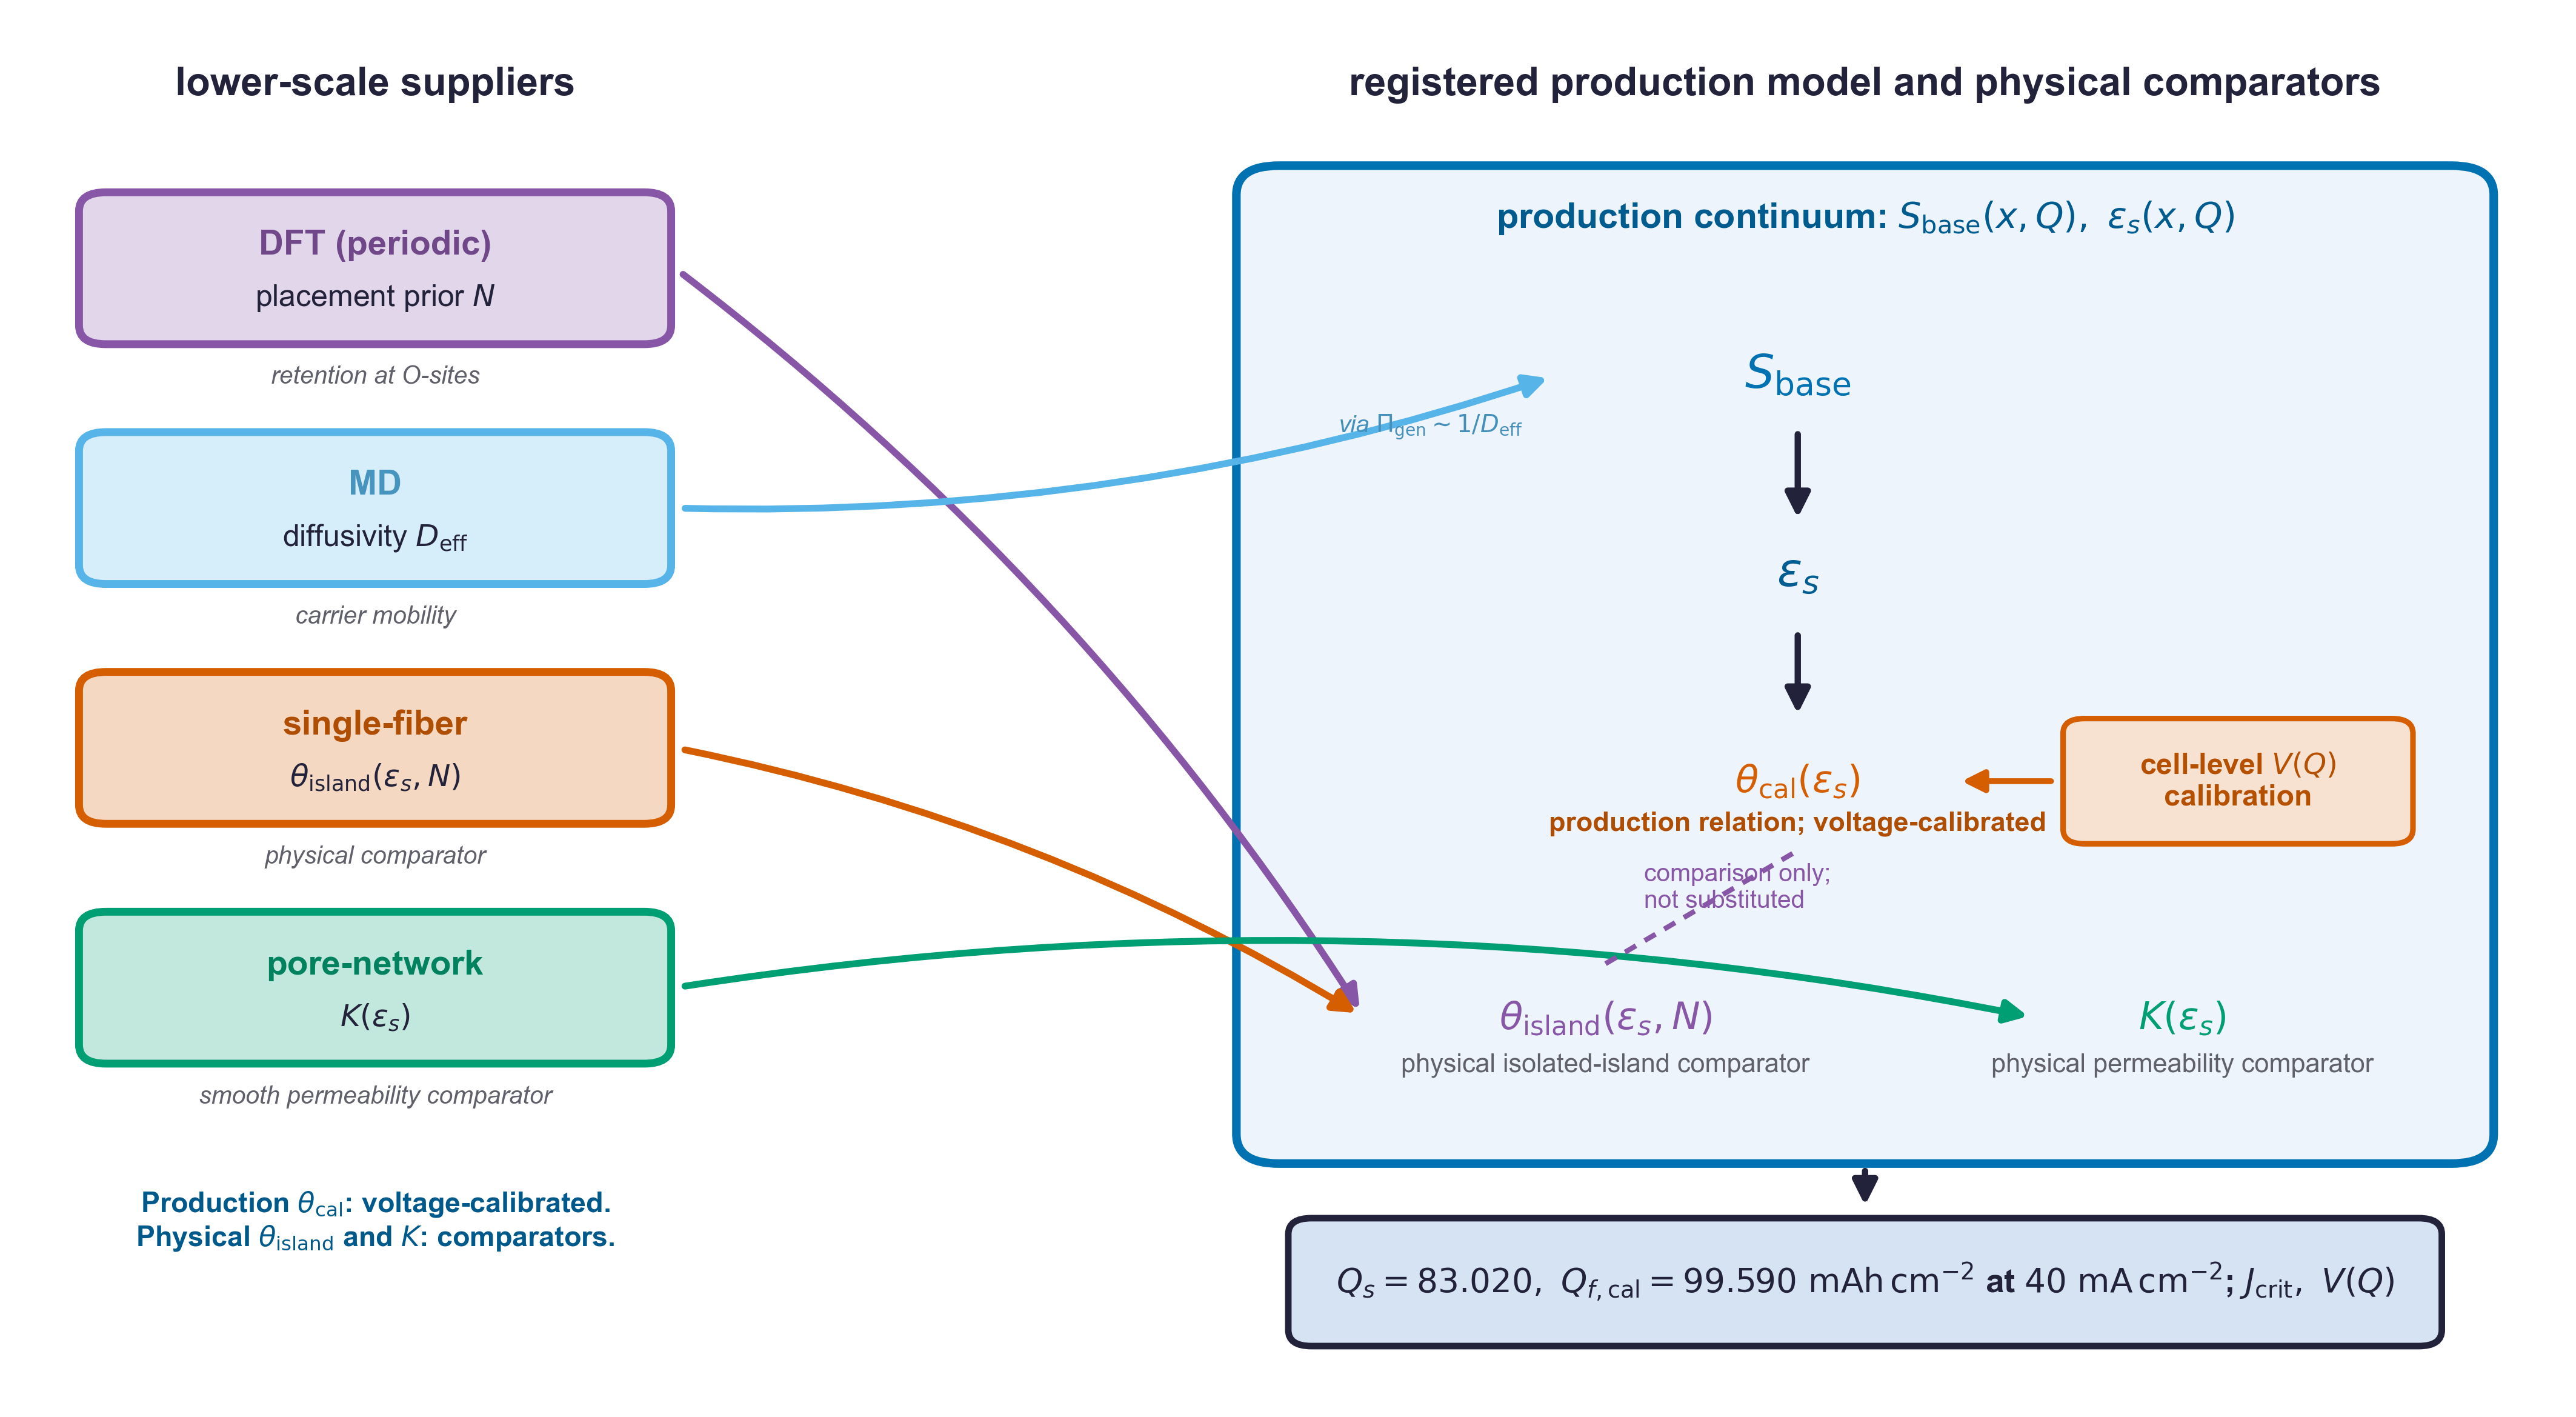
\includegraphics[width=0.90\textwidth]{figures/Fig_R568_scale_provenance.pdf}
\caption{\textbf{Evidence provenance across scales.} DFT supplies a relative placement bias; molecular
dynamics supplies a bounded bulk-carrier diffusivity prior; the single-fibre model supplies physical
isolated-island accessibility families; the pore-network model supplies a smooth relative-permeability
closure; and the continuum model supplies the spatial iodine-state fields. The production accessibility
magnitude is voltage-calibrated. Arrows are labelled by evidence type---solved field, bounded prior, physical
closure or calibrated effective closure---and do not imply a parameter-free bottom-up prediction.}
\label{fig:provenance}
\end{figure}

\subsection{Free-iodine balance and the super-saturation stress}
\label{sec:nondim}
At the carbon reaction front, the quasi-steady reduced balance across a Nernst layer of thickness $\delta$
balances the charge-equivalent supply $g=\iapp/(2F)$ against diffusive removal,
$\Deff\,\Delta\cf/\delta=g/\beta$ across the layer. Combining this balance with Eq.~\eqref{eq:beta} gives the
surface free-iodine concentration
\begin{equation}
\cf \;=\; \frac{1}{\beta}\!\left[\, c_{\mathrm{I_2,tot}} \;+\; \frac{\iapp\,\delta}{2F\,\Deff}\,\right],
\label{eq:cf}
\end{equation}
and the local super-saturation is $S=\cf/\csat^{\mathrm{eff}}$ (referenced to the effective, salting-out solubility $\csat^{\mathrm{eff}}=\csat/\gamma_{\mathrm{salt}}$; \S\ref{sec:thresh}). The reduction neglects the late
bare-versus-native-solid current partition; the native-solid path carries only $0.552\%$ of integrated charge,
although its instantaneous share rises near the endpoint (SI). Here $c_{\mathrm{I_2,tot}}$ denotes the \emph{local}
dissolved oxidized-iodine pool at the reaction front: the surface value of the solved continuum field, not
the cell-averaged inventory. When the reduced expression is projected onto a capacity axis, it uses the solved
surface trajectory, so the two terms of the bracket sit at the same location. (The balance
$\Deff\Delta\cf/\delta=g/\beta$ also takes $\beta$ as uniform across the thin layer, consistent with the fast
complexation assumption.) The bracket in Eq.~\eqref{eq:cf} is exactly the surface
variable carried by the continuum model (\S\ref{sec:multiscale}): the first term is the accumulated
oxidized-iodine inventory, the second is the generation-driven boundary-layer build-up. This buffered form
also encodes why solid \ce{I2} forms late in the production trajectory: in an iodide-rich electrolyte the
oxidation product is buffered as soluble \ce{I3^-}, so the modeled free-\ce{I2} stress increases as the local
iodide coordinate and hence $\beta$ decrease. The buffer $\beta=\beta(\ci)$ in Eq.~\eqref{eq:cf} carries this
model dependence through the solved surface-effective iodide. This is an internal state relation; the cited
electrodeposition literature documents solid iodine formation but does not verify local iodide depletion in
the present ZIFB \citep{SolidIodineElectrodeposition2025}.

\subsection{Dimensionless groups and the baseline stress}
Dividing Eq.~\eqref{eq:cf} by $\csat$ defines three dimensionless groups,
\begin{equation}
\Pi_{\mathrm{gen}} \;=\; \frac{\iapp\,\delta}{2F\,\Deff\,\csat},
\qquad
\Pi_{\mathrm{inv}} \;=\; \frac{c_{\mathrm{I_2,tot}}}{\csat},
\qquad
\beta \;\text{(Eq.~\ref{eq:beta})},
\label{eq:groups}
\end{equation}
so that the \emph{within-cycle} baseline super-saturation stress---the load-bearing coordinate of the whole
framework---is
\begin{equation}
\boxed{\;\,S_{\mathrm{base}} \;=\; \gamma_{\mathrm{salt}}\,\frac{\Pi_{\mathrm{inv}}+\Pi_{\mathrm{gen}}}{\beta_{\mathrm{intra}}(Q)}
\;=\; \frac{\cf}{\csat^{\mathrm{eff}}},
\qquad \beta_{\mathrm{intra}}\equiv\beta~(\text{Eq.~\ref{eq:beta}}),\;}
\label{eq:sbase}
\end{equation}
read at the running iodide; this is the coordinate the continuum model solves and that the two-threshold,
compression, and rate analyses below all use (throughout, ``$S$'' denotes $S_{\mathrm{base}}$ at the modeled
baseline electrolyte). Here $\Pi_{\mathrm{gen}}$ is a generation/transport Damk\"ohler number (in the spirit of
Damk\"ohler-type dimensionless reductions of flow-cell behavior \citep{DimAnalysis_CEJ2019}): the current
density (rate) and the effective diffusivity---and hence \emph{compression}, through the selected
Bruggeman-type empirical effective-medium closure $\Deff=D_0\epsl^{1.5}$---enter only here. The historical
Bruggeman framework \citep{Bruggeman1935} does not measure this exponent for the compressed graphite felt.
We quote the baseline reference value at the
free-solution reference ($\Deff\!\to\!D_0$, the Nernst layer sitting in the free electrolyte),
$\Pi_{\mathrm{gen}}\!\approx\!78$, so that compression enters as the $\epsl^{1.5}$ modifier rather than being
folded into the baseline number. The inventory group $\Pi_{\mathrm{inv}}$ carries the state of charge and the iodide inventory, and
the buffer $\beta$ falls as iodide is consumed during charge (its \emph{within-cycle} role, which the continuum
solve carries). At the modeled baseline, the registered averaged-saturation marker is
$\langle S_{\mathrm{base}}\rangle_{\mathrm{aveop1}}=1$, where the corresponding averaged free-\ce{I2}
stress reaches the effective (salting-out) reference $\csat^{\mathrm{eff}}=\csat/\gamma_{\mathrm{salt}}$
(\S\ref{sec:thresh}); the factor $\gamma_{\mathrm{salt}}$ in Eq.~\eqref{eq:sbase} converts the intrinsic-solubility
groups $\Pi$ to this effective reference, so $S_{\mathrm{base}}=\cf/\csat^{\mathrm{eff}}$ and $\Pi_{\mathrm{gen}}$
below is quoted in units of the intrinsic $\csat$. The single buffer $\beta_{\mathrm{intra}}$ captures this
within-cycle model chemistry. Cross-composition prediction is outside the registered branch; the available
NH4Br series is retained only as descriptive supporting-electrolyte context (\S\ref{sec:compmodule}).

\subsection{The positive-electrode \texorpdfstring{$J$--$Q$}{J-Q} operating boundary}
\label{sec:jq}
Because $\Pi_{\mathrm{gen}}\!\propto\!\iapp$ (the current density $J$) and
$\Pi_{\mathrm{inv}}\!\propto\!c_{\mathrm{I_2,tot}}(Q)$ (the areal capacity passed $Q$),
the baseline stress $S_{\mathrm{base}}$ is intrinsically a function of the operating point $(J,Q)$,
\begin{equation}
S_{\mathrm{base}}(J,Q)=
\gamma_{\mathrm{salt}}
\frac{\Pi_{\mathrm{inv}}(Q)+\Pi_{\mathrm{gen}}(J)}{\beta_{\mathrm{intra}}(Q)},
\qquad
\Pi_{\mathrm{gen}}(J)=\frac{J\,\delta}{2F\,\Deff\,\csat}.
\label{eq:seffjq}
\end{equation}
The two thresholds therefore trace two \emph{boundaries} in the $(J,Q)$ plane (Fig.~\ref{fig:jqmap}).
Setting $S_{\mathrm{base}}=1$ gives the saturation-marker current---the largest $J$ that, at a given $Q$,
keeps free \ce{I2} below saturation:
\begin{equation}
\boxed{\;J_s^{+}(Q)=\frac{2F\,\Deff\,\csat}{\delta}
\left[\,\frac{\beta_{\mathrm{intra}}(Q)}{\gamma_{\mathrm{salt}}}
-\Pi_{\mathrm{inv}}(Q)\right]_{+}.\;}
\label{eq:jsplus}
\end{equation}
The production accessibility relation (\S\ref{sec:thresh}) defines a closure-conditioned boundary
$J_{b,\mathrm{cal}}^{+}(Q)$ by
$\langle\thetacal(J,Q)\rangle=\tfrac12$. It lies above $J_s^{+}$ over the registered baseline trajectory,
separated from it by $\Delta Q_{\mathrm{cal}}$. A fixed-current cut returns $\Qfcal(J)$ and a fixed-capacity cut returns
$J_{b,\mathrm{cal}}^{+}(Q)$; both are projections of the calibrated model boundary. The physical-island
closure defines a different boundary and, in the matched baseline solve, does not reach half accessibility by
\SI{120}{mAh.cm^{-2}}. The experimental thickness and rate series therefore provide descriptive stress tests,
not calibration or validation of this boundary. Supporting-electrolyte composition is treated as a separate
context module in the SI so that \ce{NH4Br} does not become the organizing variable of the positive-electrode
model. Condition-labelled values of $i^{*}=2Fk$ are plotted only as external dissolution scales
(\S\ref{sec:diss}); they are not combined with $J_{b,\mathrm{cal}}^{+}$ into a ceiling for this electrolyte.

\subsection{Production state markers and physical accessibility comparators}
\label{sec:thresh}
The registered production trajectory uses two state markers:
\begin{enumerate}
\item \textbf{Baseline averaged-saturation marker}, reached at areal capacity $Q_{\mathrm s}$ at the
registered averaging-operator crossing
\[
\left\langle c_{\mathrm{I_2,surf,free}}/c_{\mathrm{I_2,sat}}\right\rangle_{\mathrm{aveop1}}=1.
\]
This is the registered positive-electrode averaging-operator crossing, not the first local supersaturation,
first auxiliary phase-transfer source or first solid. Spatially local $S>1$ can activate the native-solid path
before the electrode-average crossing. Here $\csat^{\mathrm{eff}}=\csat/\gamma_{\mathrm{salt}}$, where
$\csat=\SI{1.33}{mol.m^{-3}}$ is the dilute-water \ce{I2} solubility reference
\citep{Ramette1965} and $\gamma_{\mathrm{salt}}\approx3$ is a salting-out factor, a Setschenow-scale
reduction of neutral-\ce{I2} solubility at the electrolyte's high ionic strength, carried as a bounded prior
rather than a fitted constant and informed only by a cross-salt high-ionic-strength analogue
\citep{Palmer1984} (so $\csat^{\mathrm{eff}}\!\approx\!\SI{0.44}{mol.m^{-3}}$; SI). This factor sets
the \emph{absolute} saturation-marker scale, and the effective solubility is accordingly the second-ranked sensitivity
lever (\S\ref{sec:knob-mechanism}); the \emph{separation} of the two thresholds, by contrast, is an internal
consequence of the selected closures and is compared with distinct retained-versus-blocking physical priors
in \S\ref{sec:res-clock}.
\item \textbf{Production half-accessibility marker}, reached at $\Qfcal$, where
$\langle\thetacal(\mathbf{x},Q)\rangle=\tfrac12$. In the registered production trajectory,
$\Qfcal=\SI{99.6}{mAh.cm^{-2}}$ and $\langle\varepsilon_s\rangle=1.18572\times10^{-4}$ at that event.
This trajectory value is not a physical material threshold. The dense isolated-island half-accessibility
fraction $\varepsilon_{\mathrm{s,island},1/2}=1.7973\times10^{-3}$ and the geometric film-percolation marker
$\varepsilon_{\mathrm{s,film\text{-}perc}}^*=2.2324\times10^{-3}$ are separate physical comparators.
\end{enumerate}
The production retained-but-not-blocking interval is
$\Delta Q_{\mathrm{cal}}=\Qfcal-Q_{\mathrm s}$ and is conditional on the calibrated closure. No single
$\varepsilon_s^*$ is used across closure families. Distinct precipitation and clogging stages have physical
precedent in porous-media and electrochemical systems \citep{PorosityClog_WRR2023,ZnO_EEM2024}, while
nanoconfined solid iodine can remain electrochemically recoverable \citep{SolidI2_NatCommun2020,Fitzek2023};
these analogues motivate the separation but do not transfer a numerical threshold to the present felt.
The full COMSOL implementation accumulates native deposited solid through the super-saturation-activated Tafel
path defined below (Eq.~\ref{eq:solidode}). For the analytic operating-map reduction only, we approximate that
path by a trajectory-calibrated accumulation law. We track $\epss$ as the deposited-\ce{I2}(s) volume fraction
on the \emph{total-electrode-volume} basis throughout (consistent with the continuum closure
$\epsl=\varepsilon_0-\epss$ and the SI), so against the charge passed per electrode area
$Q_C=\int\iapp\,\mathrm{d}t$,
\begin{equation}
\frac{\mathrm{d}\epss}{\mathrm{d}Q_C} \;=\; \frac{V_m}{2F L}\,\phi_{\mathrm{ppt}}\,(S-1)_{+},
\label{eq:accum}
\end{equation}
where $V_m$ is the molar volume of \ce{I2(s)}, $L$ the electrode thickness, $(\cdot)_+$ the positive part, and
$Q_C=3.6\times10^4\,Q$ for $Q$ in $\mAhcm$. Because $\phi_{\mathrm{ppt}}$ multiplies the super-saturation
overshoot $(S-1)_+$, it is a \emph{reduced solid-formation efficiency}, not the native-path current and not a
mass-partition fraction of the total generated iodine. Its baseline value and provenance are given in the SI,
and its leverage on the production trajectory is swept in \S\ref{sec:res-sens}. The physical single-fibre
closure uses the pore-volume rescaling $\hat\epss=\epss/\epsl$, whereas the production accessibility relation
is evaluated on its own regularized solid state. In the reduced bare-path expression,
$a_{\mathrm b}\simeq a_s(1-\theta)$ with $\theta=\thetacal$ in the production branch and
$\theta=\thetaisland$ in the matched physical branch; the full implementation additionally multiplies the
bare area by $K_{\mathrm{rel}}^{1/2}$ and retains the separate native-solid path on $a_s$. A fixed-pore-occupancy scaling
$Q\propto\epsl L$ is therefore a physical comparator, not the definition of $\Qfcal$; the existing
single-cell thickness series tests only its directional plausibility.

\subsection{External dissolution-derived current scales}
\label{sec:diss}
An areal molar dissolution flux $k$ can be expressed on a two-electron current scale as
\begin{equation}
i^{*} \;=\; n F k, \qquad n=2,
\label{eq:istar}
\end{equation}
which is the dimensional conversion used by Zhao \emph{et al.}~\citep{Zhao2022}. Their reported values are
method- and iodide-concentration-dependent (\S\ref{sec:res-rate}); Eq.~\eqref{eq:istar} does not make them a
measured current ceiling for the present electrolyte.

The half-cycle distinction is essential. The measurement directly describes solid-iodine redissolution, so it
constrains discharge or rest/recovery clearance. Charge oxidizes iodide and does not require solid to dissolve;
therefore $i^{*}$ is not a direct cap on instantaneous charge current. We use it only to motivate a conditional
clearance-versus-generation hypothesis: if dissolution or complexation cannot clear oxidized iodine as quickly
as it is generated, free-iodine stress and retained inventory can increase. The production saturation marker remains
defined by Eq.~\eqref{eq:sbase}, and the production half-accessibility marker remains defined by
$\langle\thetacal\rangle=0.5$. The assumed rate laws and condition-labelled literature values are retained as
sensitivity context, not as an independently identified failure law.

\subsection{Supporting-electrolyte context}
\label{sec:compmodule}
The registered positive-electrode model is formulated at fixed
\SI{1}{M}~\ce{ZnI2}$+$\SI{4}{M}~\ce{NH4Br}. NH4Br is a representative supporting electrolyte: bromide can
participate in iodine complexation but is not the modeled faradaic protagonist, and ammonium may also affect
the negative electrode \citep{Jian2021,Park2021,Udom2025}. The available composition series has only
$1/1/1/2/1$ independent cells across 0/1/2/3/4 M and cannot identify a transferable solubility,
complexation or transport coefficient. We therefore do not propagate the previous multi-parameter
composition regression into the production boundary. Its deterministic descriptive reconstruction is reported
in the SI; prediction at a new supporting electrolyte requires independent speciation, diffusivity,
conductivity and viscosity inputs.

\section{Continuum implementation and numerical readout}
\label{sec:multiscale}
This section is the continuum implementation behind the reduced criterion: a positive-electrode porous-media
solve under full-cell boundary conditions
that turns the state variables into the spatial fields $S(x,Q)$, $\epss(x,Q)$, $\theta(x,Q)$ and the
$J$--$Q$ operating boundary. The scales play distinct, non-interchangeable roles---the continuum solve
\emph{generates} the state fields (its solved solid fraction is not itself an accessibility measure, and its
raw galvanostatic voltage is not held to experimental accuracy), the molecular and mesoscale layers provide
bounded priors or physical comparators, and the experiments have stated descriptive or calibration roles.

\begin{figure}[tbp]\centering
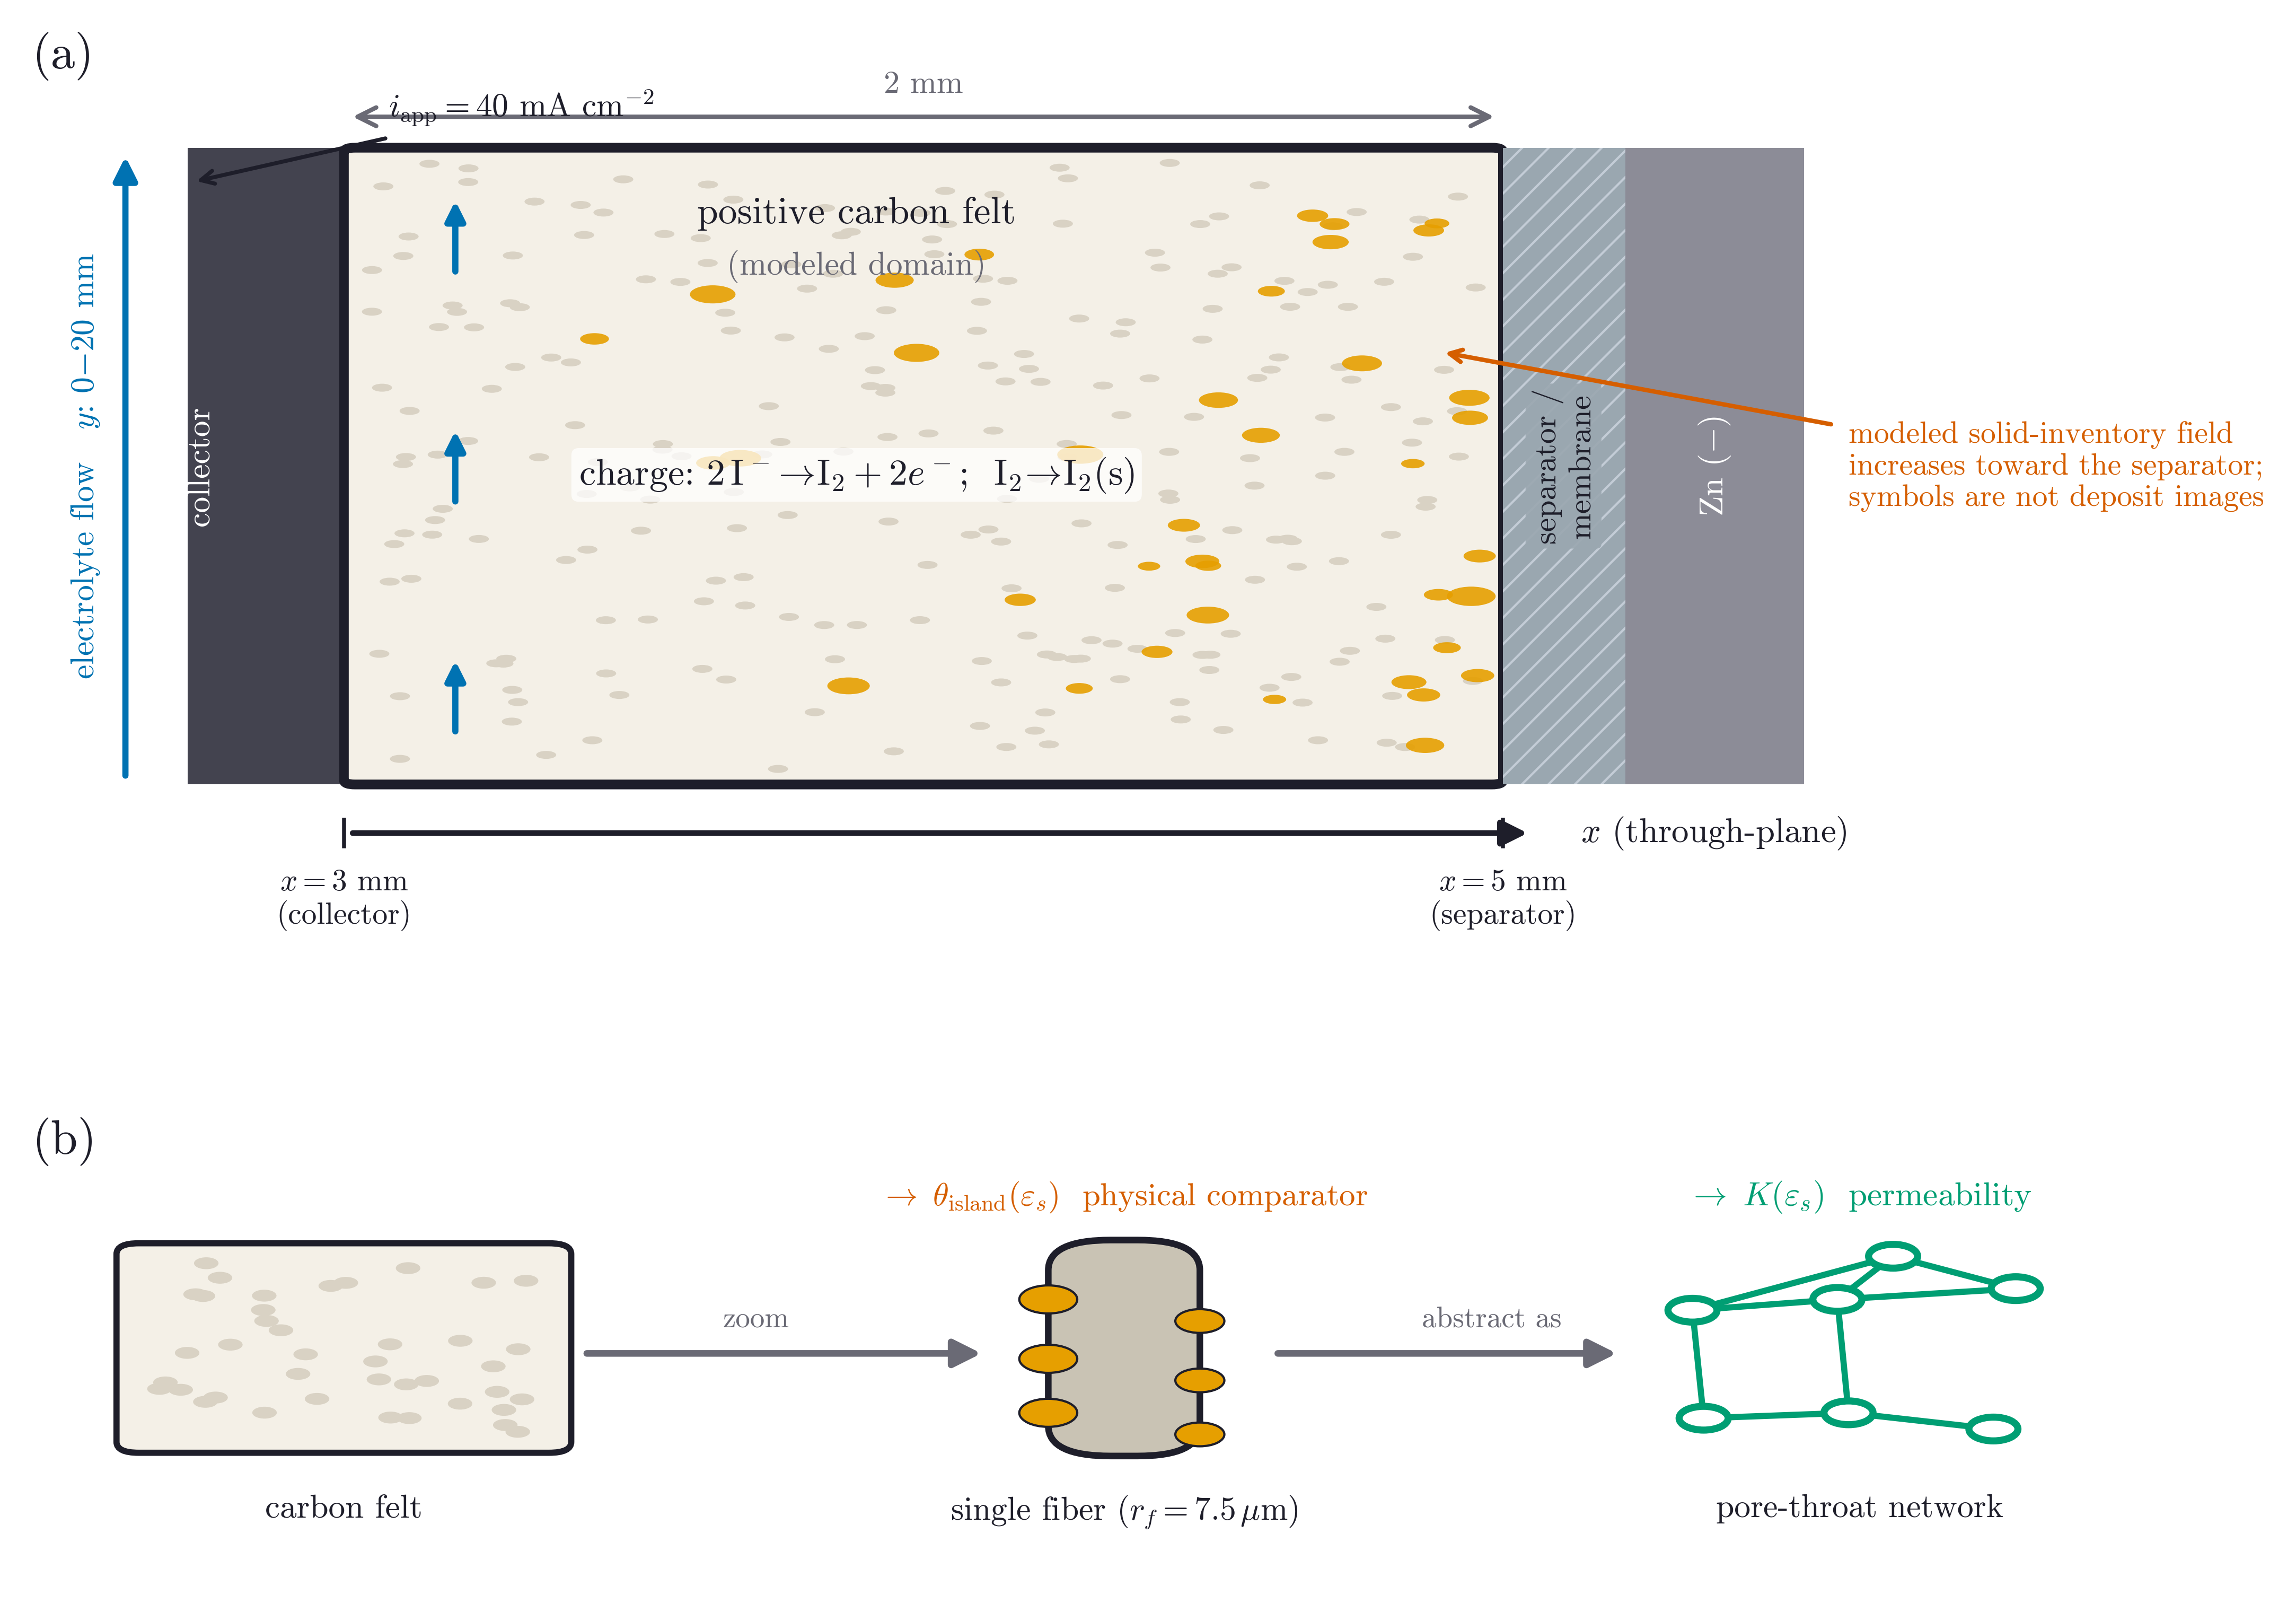
\includegraphics[width=\textwidth]{figures/Fig_R573_model_geometry.pdf}
\caption{\textbf{Modeled system and the positive-electrode domain.} (a)~The continuum model resolves the
positive carbon felt in two dimensions: a $2$\,mm-thick porous slab between the current collector
(through-plane coordinate $x=3$\,mm face) and the separator/membrane ($x=5$\,mm face, which faces the zinc
negative), with electrolyte flowing along the in-plane coordinate $y$ ($0$--$20$\,mm). Charge oxidizes iodide,
$2\,\ce{I^-}\!\rightarrow\!\ce{I2}+2e^-$; local super-saturation activates the native deposited-species path.
The schematic distinguishes soluble production, native-solid formation and accessibility loss rather than
asserting a resolved morphology. Orange symbols schematize retained inventory and are not deposit images
or a morphology assignment. The solve returns the through-plane fields $S$, $\epss$, the selected $\theta$, the flow velocity and the
current; the maps of Fig.~\ref{fig:evolution} and Supplementary Fig.~\ref{fig:spatial} are slices of this same domain
(Fig.~\ref{fig:evolution} averaged over $y$). (b)~The mesoscale models provide physical comparators: a
single-fiber unit cell ($r_f=7.5$\,$\mu$m) supplies the isolated-island family
$\thetaisland(\epss,N)$, and a pore-throat network supplies the smooth-permeability response $K(\epss)$.
Neither fixes the voltage-calibrated production magnitude.}
\label{fig:geometry}
\end{figure}

A positive-electrode continuum solve under full-cell boundary conditions tests the dimensionless theory and
integrates its closures. The modeled domain is
the positive carbon felt (Fig.~\ref{fig:geometry}): a $2$\,mm-thick porous slab resolved in two dimensions,
with the through-plane coordinate $x$ running from the current-collector face to the separator/membrane face
(which faces the zinc negative) and the in-plane coordinate $y$ ($0$--$20$\,mm) along the electrolyte flow; the
reaction current and modeled solid inventory are nonuniform across the through-plane domain. These are
continuum fields, not a resolved deposit geometry. A tertiary-current-distribution model \citep{Newman1962,Tichter2020,Chakrabarti2020,AparicioMauricio2023} solves the
governing balances of \S\ref{sec:backbone} (Eqs.~\eqref{eq:cR}--\eqref{eq:feedback}) in the real cell
geometry, with two-way Darcy/porous-media flow: the velocity is solved and coupled back into
transport, and the permeability feedback stays mild within the analyzed window (\S\ref{sec:perm}).
The solve includes a constant-exchange-current Butler--Volmer soluble-iodine path, an empirical
oxidized-pool Nernst-like equilibrium potential, and a local-super-saturation-activated native-solid Tafel
path for the same overall $2\,\ce{I^-}\rightarrow\ce{I2}+2e^-$ couple. The native-solid path, not the
parallel auxiliary phase-transfer tracker, advances the deposited-species volume used by the accessibility,
permeability and transport closures of \S\ref{sec:closures}. The reported model
terminal voltage is the solved galvanostatic scaffold response, not an empirical fit or an independently
validated full-cell prediction; numerical details are in the Methods.
For \emph{interpreting} the voltage we additionally use a Butler--Volmer reduction,
\begin{equation}
V(Q)=V_0+\underbrace{\frac{RT}{2F}\ln\!\left(\frac{\cf}{c_{\mathrm{obs}}^{\circ}}\right)}_{\text{concentration term}}
      +\, b_T\!\left[\underbrace{\ln\!\frac{\ci^0}{\ci(Q)}}_{\text{iodide depletion}}
      +\underbrace{\ln\!\frac{1}{A_{\mathrm{bare}}(Q)}}_{\text{accessibility}}\right]+\iapp R_\Omega,
\label{eq:vred}
\end{equation}
where $c_{\mathrm{obs}}^{\circ}=\SI{1}{mol.m^{-3}}$ makes the logarithm dimensionless (a different reference is
absorbed into $V_0$). Here $V_0$ and the apparent Tafel-like coefficient $b_T$ are fitted observation-layer
coefficients, not independently identified physical kinetic parameters.

\subsection{Governing balances of the positive-electrode scaffold}
\label{sec:backbone}
The reduced criterion of \S\ref{sec:theory} distills a continuum iodine-state scaffold; we state its minimal
closed set here so that the baseline stress $S_{\mathrm{base}}$ reads as a consequence of an explicit
porous-electrode balance rather than an assertion. The full implementation (advective transport, reservoir and
boundary conditions, parameter provenance) is given in the SI. The solved pore-phase species is the lumped
oxidized pool $c_O$ (internal field \texttt{cBr2}); the free-iodide coordinate is an algebraic inventory,
\begin{align}
c_R &= \max\!\left(c_{R,\mathrm{floor}},c_{R,0}-3c_O\right), \label{eq:cR}\\
\varepsilon_0\,\partial_t c_O+\nabla\!\cdot
\left(\mathbf{u}c_O-D_{O,\mathrm{eff}}\nabla c_O\right)
&=R_{\mathrm b}-R_{\mathrm{dep}}+\frac{r_{\mathrm d}-r_{\mathrm p}}{V_m}. \label{eq:cO}
\end{align}
Here $R_{\mathrm b}=a_{\mathrm b}j_{\mathrm b}/(2F)$ is soluble-iodine production on accessible carbon,
$R_{\mathrm{dep}}=a_sj_{\mathrm{dep}}/(2F)$ is conversion into the native deposited species, and
$r_{\mathrm p},r_{\mathrm d}$ are the much smaller auxiliary volume-fraction rates defined below. The factor
three in Eq.~\eqref{eq:cR} is the registered stoichiometric inventory closure for oxidation plus triiodide
binding; it is not a second transported-species equation. Charge is conserved through the sum of the two
positive-electrode paths,
\begin{equation}
\begin{aligned}
i_v&=a_{\mathrm b}j_{\mathrm b}+a_sj_{\mathrm{dep}},\\
\nabla\!\cdot\mathbf{i}_s&=-i_v, & \mathbf{i}_s&=-\sigma_{s,\mathrm{eff}}\nabla\phi_s,\\
\nabla\!\cdot\mathbf{i}_l&=+i_v, & \mathbf{i}_l&=-\kappa_{l,\mathrm{eff}}\nabla\phi_l.
\end{aligned}
\label{eq:charge}
\end{equation}
The bare-carbon path uses a constant prescribed exchange-current density; concentration enters through the
implemented equilibrium-potential expression rather than through reaction orders,
\begin{equation}
\begin{aligned}
j_{\mathrm b} &= i_0\!\left[e^{\alpha_a F\eta/RT}-e^{-\alpha_c F\eta/RT}\right],\\
\eta&=\phi_s-\phi_l-E_{\mathrm{eq}},\\
E_{\mathrm{eq}}&=E^{0\prime}+\gamma_a\frac{RT}{2F}\ln\!\left[
\frac{\max(\cf,c_{\mathrm f})}{c_{\mathrm{ref}}/\beta}\right]+\eta_{\mathrm{tank}},\\
a_{\mathrm b}&=a_s(1-\theta)K_{\mathrm{rel}}^{1/2}.
\end{aligned}
\label{eq:bv}
\end{equation}
The registered values are $i_0=5\times10^{4}~\si{A.m^{-2}}$, $\alpha_a=\alpha_c=1$,
$E^{0\prime}=\SI{0.548}{V}$, $c_{\mathrm{ref}}=\SI{120}{mol.m^{-3}}$,
$c_{\mathrm f}=\SI{0.02}{mol.m^{-3}}$ and $\gamma_a=1$. Because $\cf=c_O/\beta$, the $\beta$ terms cancel
away from the numerical floor; Eq.~\eqref{eq:bv} is therefore an empirical total-oxidized-pool Nernst-like
potential, not a full activity model for the \ce{I2}/\ce{I^-} couple. The tank correction switches on only
after the registered charge window and is zero for the results reported here.

The native-solid path uses COMSOL's anodic Tafel form and is activated by the \emph{local} free-iodine stress,
\begin{equation}
\begin{aligned}
j_{\mathrm{dep}}&=i_{0,\mathrm{dep}}\,10^{\eta/A_a}, &
i_{0,\mathrm{dep}}&=i_{0,\mathrm{dep}}^{\mathrm{base}}\max(S_{\mathrm{local}}-1,0),\\
\partial_t\epss&=V_mR_{\mathrm{dep}}, &
\partial_t\varepsilon_{\mathrm{s,aux}}&=r_{\mathrm p}-r_{\mathrm d},\qquad
\partial_tN_{\mathrm{I_2}}=\kappa_N(N_{\mathrm{target}}-N_{\mathrm{I_2}}).
\end{aligned}
\label{eq:solidode}
\end{equation}
Here $i_{0,\mathrm{dep}}^{\mathrm{base}}=\SI{0.05}{A.m^{-2}}$ and $A_a=\SI{118}{mV}$. The deposited
species $\epss$ in Eq.~\eqref{eq:solidode} is the inventory used by every transport and accessibility closure.
The parallel smooth phase-transfer state $\varepsilon_{\mathrm{s,aux}}$ reaches
$1.08\times10^{-6}$ at the endpoint and enters the $c_O$ balance only through
$(r_{\mathrm d}-r_{\mathrm p})/V_m$; it does not drive $N_{\mathrm{I_2}}$. The latter evolves in parallel by
its own target-relaxation equation and enters the calibrated accessibility relation. By comparison,
$\epss=3.219\times10^{-3}$ for the native deposited species. The deposited path carries $0.552\%$ of the
integrated charge but $28.0\%$ of the endpoint positive current. Local activation before the electrode-average
$S=1$ crossing makes $Q_{\mathrm s}$ an averaged saturation coordinate rather than a first-solid event. The solid
feeds back on transport only through algebraic closures,
\begin{equation}
\begin{aligned}
\epsl&=\varepsilon_0-\epss, &
\{D,\kappa_l\}&\propto\Big(\tfrac{\epsl}{\varepsilon_0}\Big)^{3/2},\\
K&=\Big(\tfrac{\epsl}{\varepsilon_0}\Big)^{3}
\Big(\tfrac{1-\varepsilon_0}{1-\epsl}\Big)^{2}, &
\theta&=\mathcal{C}_{b}(\epss),
\end{aligned}
\label{eq:feedback}
\end{equation}
with $\varepsilon_0$ the felt porosity, $\epsl$ the running pore-liquid fraction (Table~\ref{tab:notation}),
$K$ the relative permeability, and $\mathcal{C}_{b}$ the registered branch-specific accessibility relation:
$\thetacal$ for production or $\thetaisland$ for the dense physical comparator. The headline relation
$\Deff=D_0\epsl^{1.5}$ thus carries the full Bruggeman modifier $\epsl^{1.5}$ on the
free diffusivity (the baseline $\Pi_{\mathrm{gen}}$ below is quoted at $\Deff\!\to\!D_0$). That modifier
factors as $\epsl^{1.5}=\varepsilon_0^{1.5}(\epsl/\varepsilon_0)^{3/2}$ into a felt-porosity part
$\varepsilon_0^{1.5}$ that responds to \emph{compression} and a residual $(\epsl/\varepsilon_0)^{3/2}$ that
responds to native-solid \emph{loading}.

Of these, $c_O,\phi_s,\phi_l,\epss,\varepsilon_{\mathrm{s,aux}}$ and $N_{\mathrm{I_2}}$ are solved states;
$c_R,\epsl,D,\kappa_l,K$ and $\theta$ are algebraic consequences or closures evaluated on them; and the
super-saturation $S$ with the dimensionless groups of
\S\ref{sec:nondim} is the reduced coordinate read off the solved state. This separation is made explicit in
the model stack and the implementation-to-theory map of the SI. Convection enters as
a solved Darcy/porous-media field whose velocity is computed and fed back into transport (full two-way
coupling). In practice this feedback is negligible because native-solid loading barely lowers the permeability
before failure (\S\ref{sec:perm}): the solved velocity varies by $<\!0.1\%$ across a charge, and a
frozen-velocity control gives the same saturation marker within the reported numerical tolerance. Finally,
integrating both faradaic paths across the thickness gives
$\tfrac{1}{2F}\!\int_0^L(a_{\mathrm b}j_{\mathrm b}+a_sj_{\mathrm{dep}})\,\mathrm{d}x=\iapp/2F$.
The reduced $\Pi_{\mathrm{gen}}$ uses this total charge-equivalent supply and carries no explicit $a_sL$ factor;
its interpretation as soluble-pool generation is an approximation bounded by the $0.552\%$ integrated
native-solid-path share.

The model's assumption-to-claim boundaries are consolidated in Supplementary Table~\ref{tab:bounds}. The
release-critical distinctions are that the positive electrode is solved while the zinc electrode is not;
speciation and the Nernst layer are reduced closures; $\epss$ is an inventory rather than an accessibility
measurement; production $\thetacal$ is calibrated; physical $\thetaisland$ is a separate morphology-prior
family; and $i^{*}=2Fk$ is a condition-labelled external scale rather than a present-cell ceiling.

Taken together, these scales form an evidence map rather than a parameter-free chain: each calculation has a
registered role in the reduced continuum criterion or its physical bounds (Fig.~\ref{fig:provenance}). This
makes explicit what each scale is \emph{for}: DFT supplies only a relative placement tendency, not the island
density $N$; MD supplies a bounded oxidized-carrier diffusivity prior; and the single-fiber and pore-network
calculations bound physical accessibility and smooth-permeability responses. The voltage-calibrated
production relation remains a separate model object. Its implementation-to-theory map is tabulated in the SI.

\section{Results}
\label{sec:results}
The results are organized around one question---\emph{when does soluble or retained iodine become associated
with modeled loss of positive-electrode accessibility?} We first resolve a registered production charge
(\S\ref{sec:res-clock}), then isolate the information added by the accessibility closure
(\S\ref{sec:res-ablation}). Molecular calculations provide placement and diffusivity priors
(\S\ref{sec:res-mol}); single-fiber and pore-network calculations provide distinct physical bounds
(\S\ref{sec:res-meso}); matched continuum solves quantify model-form sensitivity without assigning a unique
deposit morphology. We then map the conditional operating envelope (\S\ref{sec:res-sens}), compare it with
condition-labelled dissolution kinetics (\S\ref{sec:res-rate}), bound alternative transport channels
(\S\ref{sec:perm}), and rank model-internal levers (Table~\ref{tab:knobs},
\S\ref{sec:knob-mechanism}).

\paragraph{What the model does and does not predict.}
Four results are carried forward with explicit evidence labels. (i)~Within the registered production branch,
the registered averaged-saturation marker precedes the voltage-calibrated half-accessibility marker. (ii)~The resulting interval
$\Delta Q_{\mathrm{cal}}$ is a closure-conditioned model output, not a universal reserve. (iii)~Published
iodine-dissolution measurements provide an external, method- and concentration-dependent kinetic scale; they
do not independently determine the sustainable current of the present electrolyte. (iv)~The sensitivity
analysis identifies model-internal directions and dominant priors, while absolute capacities remain conditional
on $\csat$, $\Deff$, $\gamma_{\mathrm{salt}}$ and the accessibility closure. Cycle-level reset and deposit
identity are outside the solved single charge (\S\ref{sec:scope}).

\subsection{The registered production charge: saturation, retention, and calibrated accessibility}
\label{sec:res-clock}
The load-bearing production-model result is the separation between the saturation marker
$Q_{\mathrm s}=\SI{83.0}{mAh.cm^{-2}}$ and the calibrated half-accessibility marker
$\Qfcal=\SI{99.6}{mAh.cm^{-2}}$, giving
$\Delta Q_{\mathrm{cal}}=\SI{16.6}{mAh.cm^{-2}}$. These are events on the registered
\texttt{PB-R526-J40-Q120-DSET5-v1} trajectory and are not physical-island thresholds or experimental
landmarks. The production solve separates quantities that an iodine-inventory metric would merge: averaged
free-\ce{I2} saturation, retained solid, and the response of the calibrated accessibility state
(Table~\ref{tab:clock}, Fig.~\ref{fig:evolution}). The positive-electrode \texttt{aveop1} stress crosses $S=1$ at
$Q_{\mathrm s}$, about $40\%$ positive-electrode state of charge. Native-solid-path current is non-zero at every
resolved node by $Q=96$, where the volume-averaged $\epss$ is $7.13\times10^{-5}$; these are solver readouts,
not experimental solid-formation detections. The correspondingly averaged production response reaches
$\langle\thetacal\rangle=0.5$ and $0.9$ at $Q=99.6$ and $\SI{111.2}{mAh.cm^{-2}}$, respectively, and its
modeled $\mathrm{d}V/\mathrm{d}Q$ maximum follows at $\SI{116.7}{mAh.cm^{-2}}$. One half is a declared
midpoint of the calibrated accessibility response, not a universal percolation threshold or an identified
morphological transition. The alternative 0.01 and 0.9 criteria are reported only to show criterion
sensitivity.
Quantitatively, the production generation group is $\Pi_{\mathrm{gen}}=77.9$ (at the free-diffusivity reference
so that compression enters as the $\Deff=D_0\epsl^{1.5}$ modifier). At $Q=0$ the stored oxidized inventory is
negligible, so the initial surface total ($78.0$ in units of $\csat$) \emph{is} this generation term rather
than pre-existing iodine. Over the charge the total oxidized-iodine inventory rises $4.16\times$
while the \emph{free}, precipitable fraction rises $9.48\times$, because iodide is consumed $58\%$ and the
buffer collapses from $\beta=1263$ to $554$. In aqueous polybromide catholytes, separate-phase or vapor
bromine emergence is state-of-charge- and complexant-dependent \citep{Choi2024}. In a distinct static
Zn--\ce{I2}/KB cell, in-situ UV--visible spectroscopy shows the dissolved \ce{I3^-} concentration rising
sharply near $1.45$~V \citep{ChenACSEnergyLett2024}. These observations are chemistry-specific analogues, not
confirmation of free-halogen emergence in the present ZIFB. The as-solved two-dimensional field maps
(Supplementary Fig.~\ref{fig:spatial})
and the through-plane space-time evolution (Fig.~\ref{fig:evolution}) make this concrete: solid \ce{I2} and the
total current localize in a thin band at one electrode face while the free-\ce{I2} stress remains a smooth
gradient, and the calibrated accessibility-loss region builds at that face as capacity increases. That the reduced stress
$S_{\mathrm{base}}$ reads back the solver's exported super-saturation channel up to a single known
normalization (slope $3.00$, from the free-monomer reference $\csat/3$) is an algebraic consistency check
(SI), not an independent validation.

\begin{table}[!htb]\centering\small
\caption{\textbf{Registered production-state events and criterion sensitivity.} Model outputs for the
registered $J=\SI{40}{mA.cm^{-2}}$ production charge. The $\thetacal$ criteria are readouts of the calibrated
production relation and are not physical-island or experimental thresholds.}
\label{tab:clock}
\begin{tabular}{@{}p{0.22\linewidth}p{0.25\linewidth}p{0.13\linewidth}p{0.23\linewidth}@{}}
\toprule
event & criterion & $Q$ (\si{\mAhcm}) & meaning \\
\midrule
averaged-saturation marker & $\langle S\rangle_{\mathrm{aveop1}}=1$ & $83$ & registered mean free-\ce{I2}
stress reaches unity; not first local solid \\
first production-accessibility response & $\langle\thetacal\rangle=0.01$ (criterion-sensitivity entry) & $85$ &
earliest response under the calibrated closure, near the resolution floor \\
native solid finitely resolved & solid-path current at every node; averaged $\epss=7.13\times10^{-5}$ & $96$ &
retained \ce{I2}(s) registered throughout the positive domain \\
production half-accessibility marker & $\langle\thetacal\rangle=\tfrac12$ ($\equiv\Qfcal$) & $99.6$ & declared
midpoint of the calibrated response \\
production high-accessibility-loss marker & $\langle\thetacal\rangle=0.9$ & $111.2$ & criterion-sensitivity
readout \\
voltage symptom & $\mathrm{d}V/\mathrm{d}Q$ peak & $116.7$ & downstream observable \\
\bottomrule
\end{tabular}
\end{table}

\begin{figure}[tbp]\centering
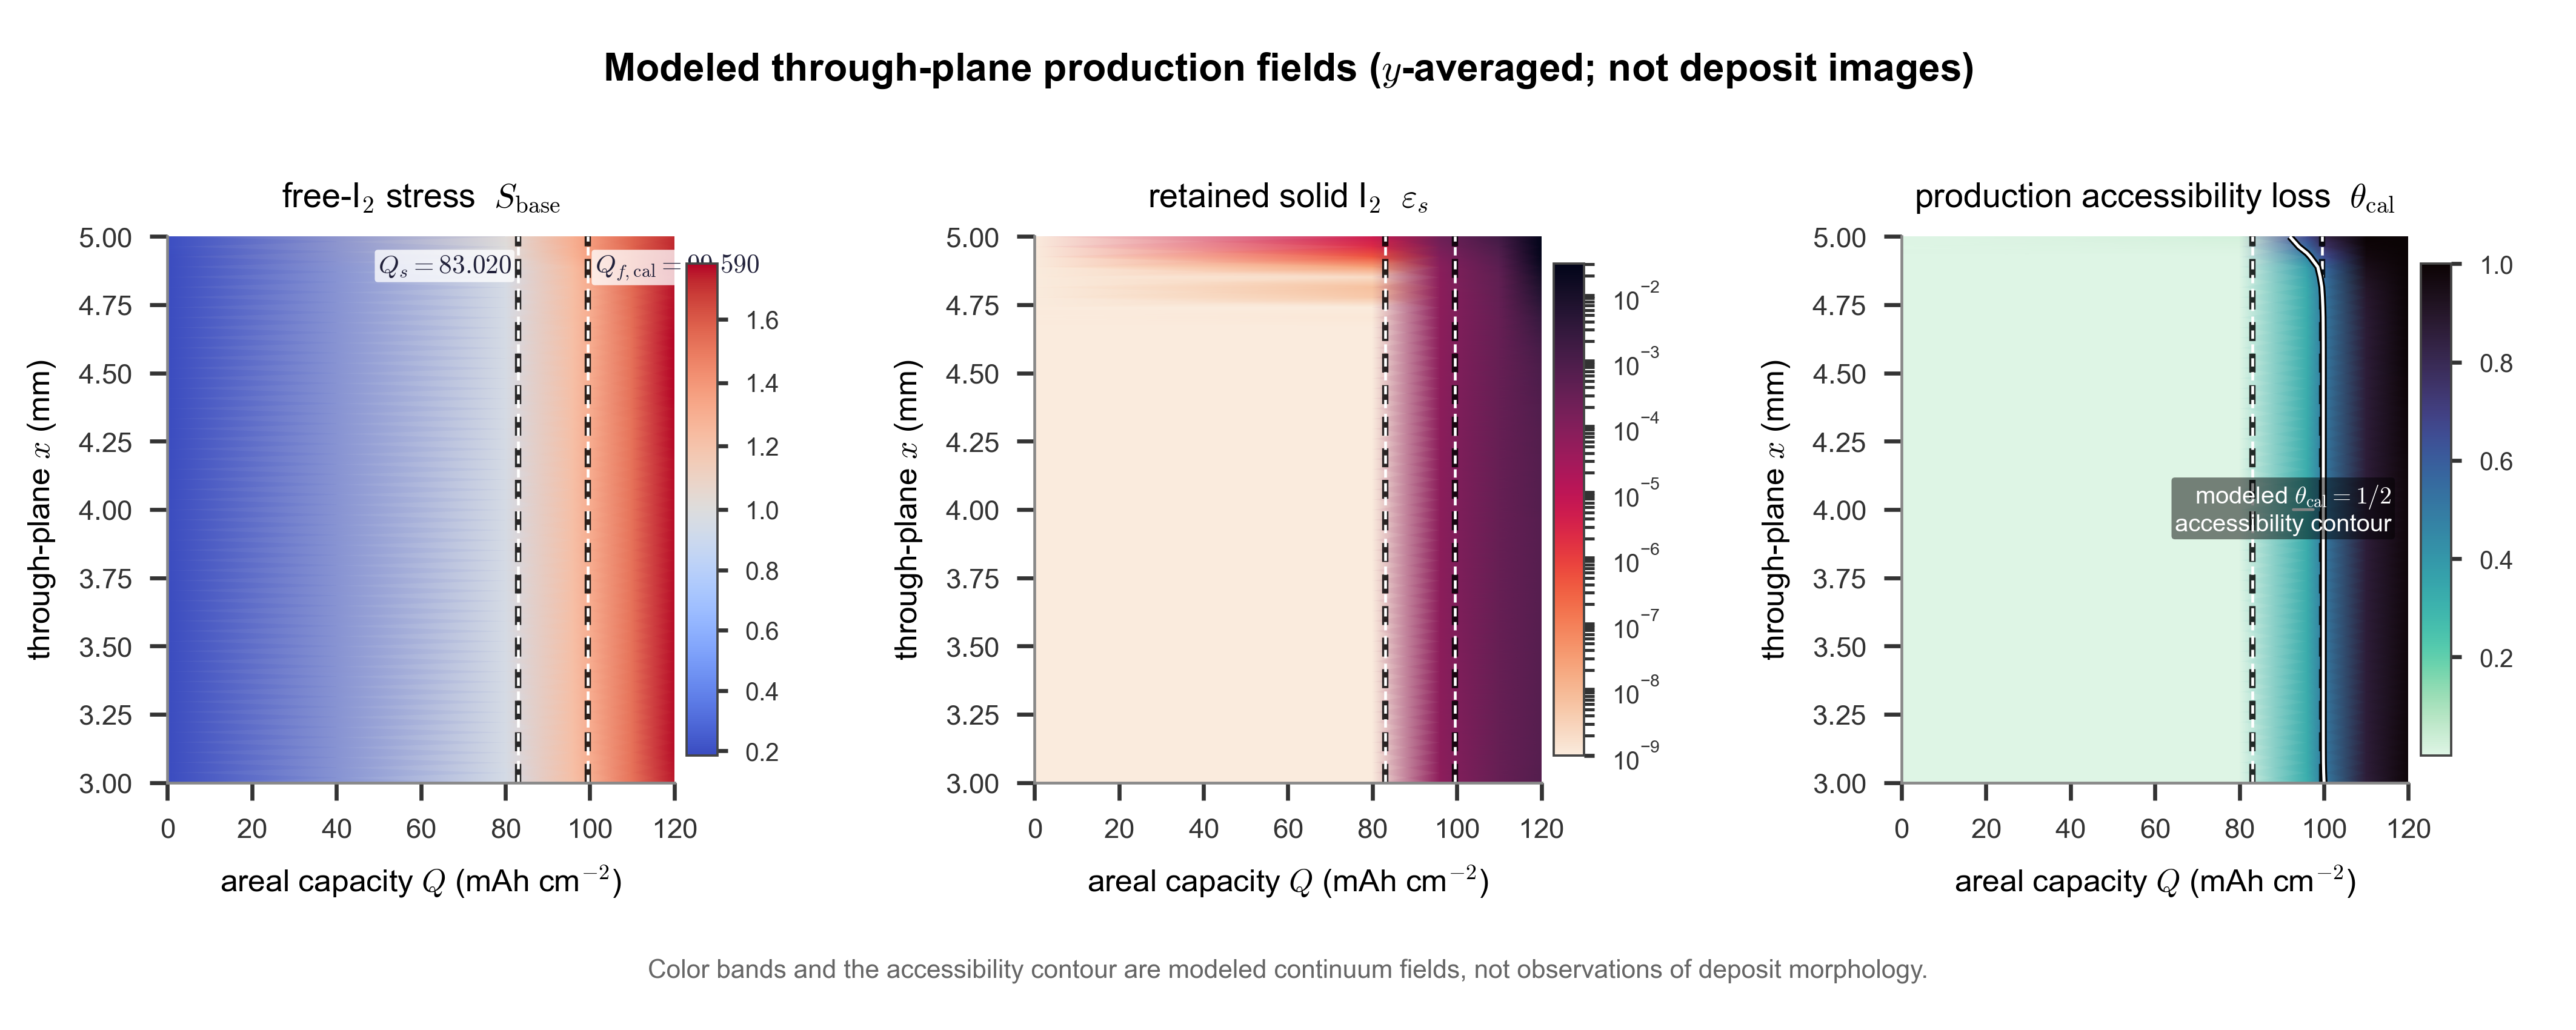
\includegraphics[width=0.98\textwidth]{figures/Fig_R545_xQ_evolution.pdf}
\caption{\textbf{Through-plane evolution of the registered production state.} Each panel is a field from the 2D domain of
Fig.~\ref{fig:geometry}, averaged over the flow direction $y$ and plotted against through-plane position $x$
(vertical; collector at $3$\,mm, separator at $5$\,mm) and areal capacity passed $Q$ (horizontal, the
charge ``clock''). Left to right: free-\ce{I2} stress $S$, retained solid fraction $\epss$, and calibrated
accessibility loss $\thetacal$. The dashed verticals mark the production saturation marker
$Q_{\mathrm s}=83.0$ and calibrated half-accessibility marker $\Qfcal=99.6~\si{mAh.cm^{-2}}$
(Table~\ref{tab:clock}). The stress rises smoothly; retained solid is concentrated near the separator-facing
side; and the production-closure half-accessibility contour develops there first. The contour is a solved
state of the calibrated closure, not an observed blocking front or an identified deposit morphology.}
\label{fig:evolution}
\end{figure}

\paragraph{The native-solid path and the surviving bare-carbon path retain partial spatial overlap.}
We re-exported the true partial currents directly from the registered \texttt{dset5}$\rightarrow$\texttt{sol5}
branch at six capacities and 5995 positive-domain nodes per snapshot. The exported arealized partial currents are
$J_{\mathrm b}^{A}=W_{\mathrm{cf}}a_{\mathrm b}j_{\mathrm b,loc}$ for the bare-carbon path and
$J_{\mathrm{dep}}^{A}=W_{\mathrm{cf}}a_sj_{\mathrm{dep,loc}}$ for the native-solid path, where
$W_{\mathrm{cf}}$ is the \SI{2}{mm} felt thickness. The latter is
non-zero at every exported node by $Q=\SI{96}{\mAhcm}$. At $Q=120$, define the ``solid-rich half'' as the
unweighted exported nodes above the within-snapshot median $\epss$. On that descriptive point-sampling basis,
$98.6\%$ of the native-solid-current magnitude and $84.3\%$ of the bare-path-current magnitude fall in that
half. The closure-defined bare area is, by construction, anti-correlated with retained solid (Spearman
$\rho=-0.99$), while the intensive bare-carbon rate (among the 5615 nodes with $a_{\mathrm b}>0$) and
native-solid current have positive rank correlations with solid ($\rho=+0.96$ and $+0.96$); the extensive
bare-path current has only a weak positive rank correlation
($\rho=+0.20$). Its raw Pearson coefficient has the opposite sign ($r=-0.21$). Because these exported points
carry no quadrature weights and the summaries are metric-dependent, neither sign is used to infer general
exclusion or a morphology. A separate positive-electrode averaging-operator ledger gives a native-solid-path
share of $28.0\%$ at the endpoint but only $0.552\%$ integrated over the full charge. Thus the spatial table is
a descriptive readout of the imposed accessibility closure, not independent validation of blocking. The frozen
node table and analysis are included in the release source data.

\subsection{An accessibility closure adds information and changes the coupled trajectory}
\label{sec:res-ablation}
The ablation is a bookkeeping test on the production state (Fig.~\ref{fig:ablation}). The stress $S$ identifies
the modeled saturation crossing but contains no accessibility state; $\epss$ records retained inventory but
contains no declared functional criterion. The calibrated relation $\thetacal(\epss)$ maps that inventory to
the production accessibility response, including $\Qfcal$. Thus $S$, $\epss$, $\thetacal$ and
$A_{\mathrm{bare}}=1-\thetacal$ carry distinct information on one capacity axis. This does not make
$\langle\thetacal\rangle=0.5$ a physical percolation threshold, nor does it identify $N$: the physical
isolated-island response and its half-accessibility fraction are analyzed separately. The same
inventory--current decoupling is observed directly across published cells: at fixed iodine inventory the
deliverable capacity collapses about five-fold when the current density is raised five-fold and recovers
fully on returning to the low rate \citep{LiDualPlate2025}. In one biphasic Zn--I system, pushing iodine
concentration from the robust $1.7$--$2.2$~M range to $2.7$~M worsened rate stability
\citep{ZnI_EES2025}; reducing loading extended high-rate cycling in a separate design
\citep{ShakeriHosseinabad2023}. Together these reports show that stored amount alone does not fix high-rate
utilization; they do not establish a universal current ceiling for the present electrode. The
next two subsections provide bounded molecular and mesoscale priors for $\Deff$, physical island accessibility
and $K(\epss)$; they do not bottom-up determine the calibrated production magnitude.

\begin{figure}[tbp]\centering
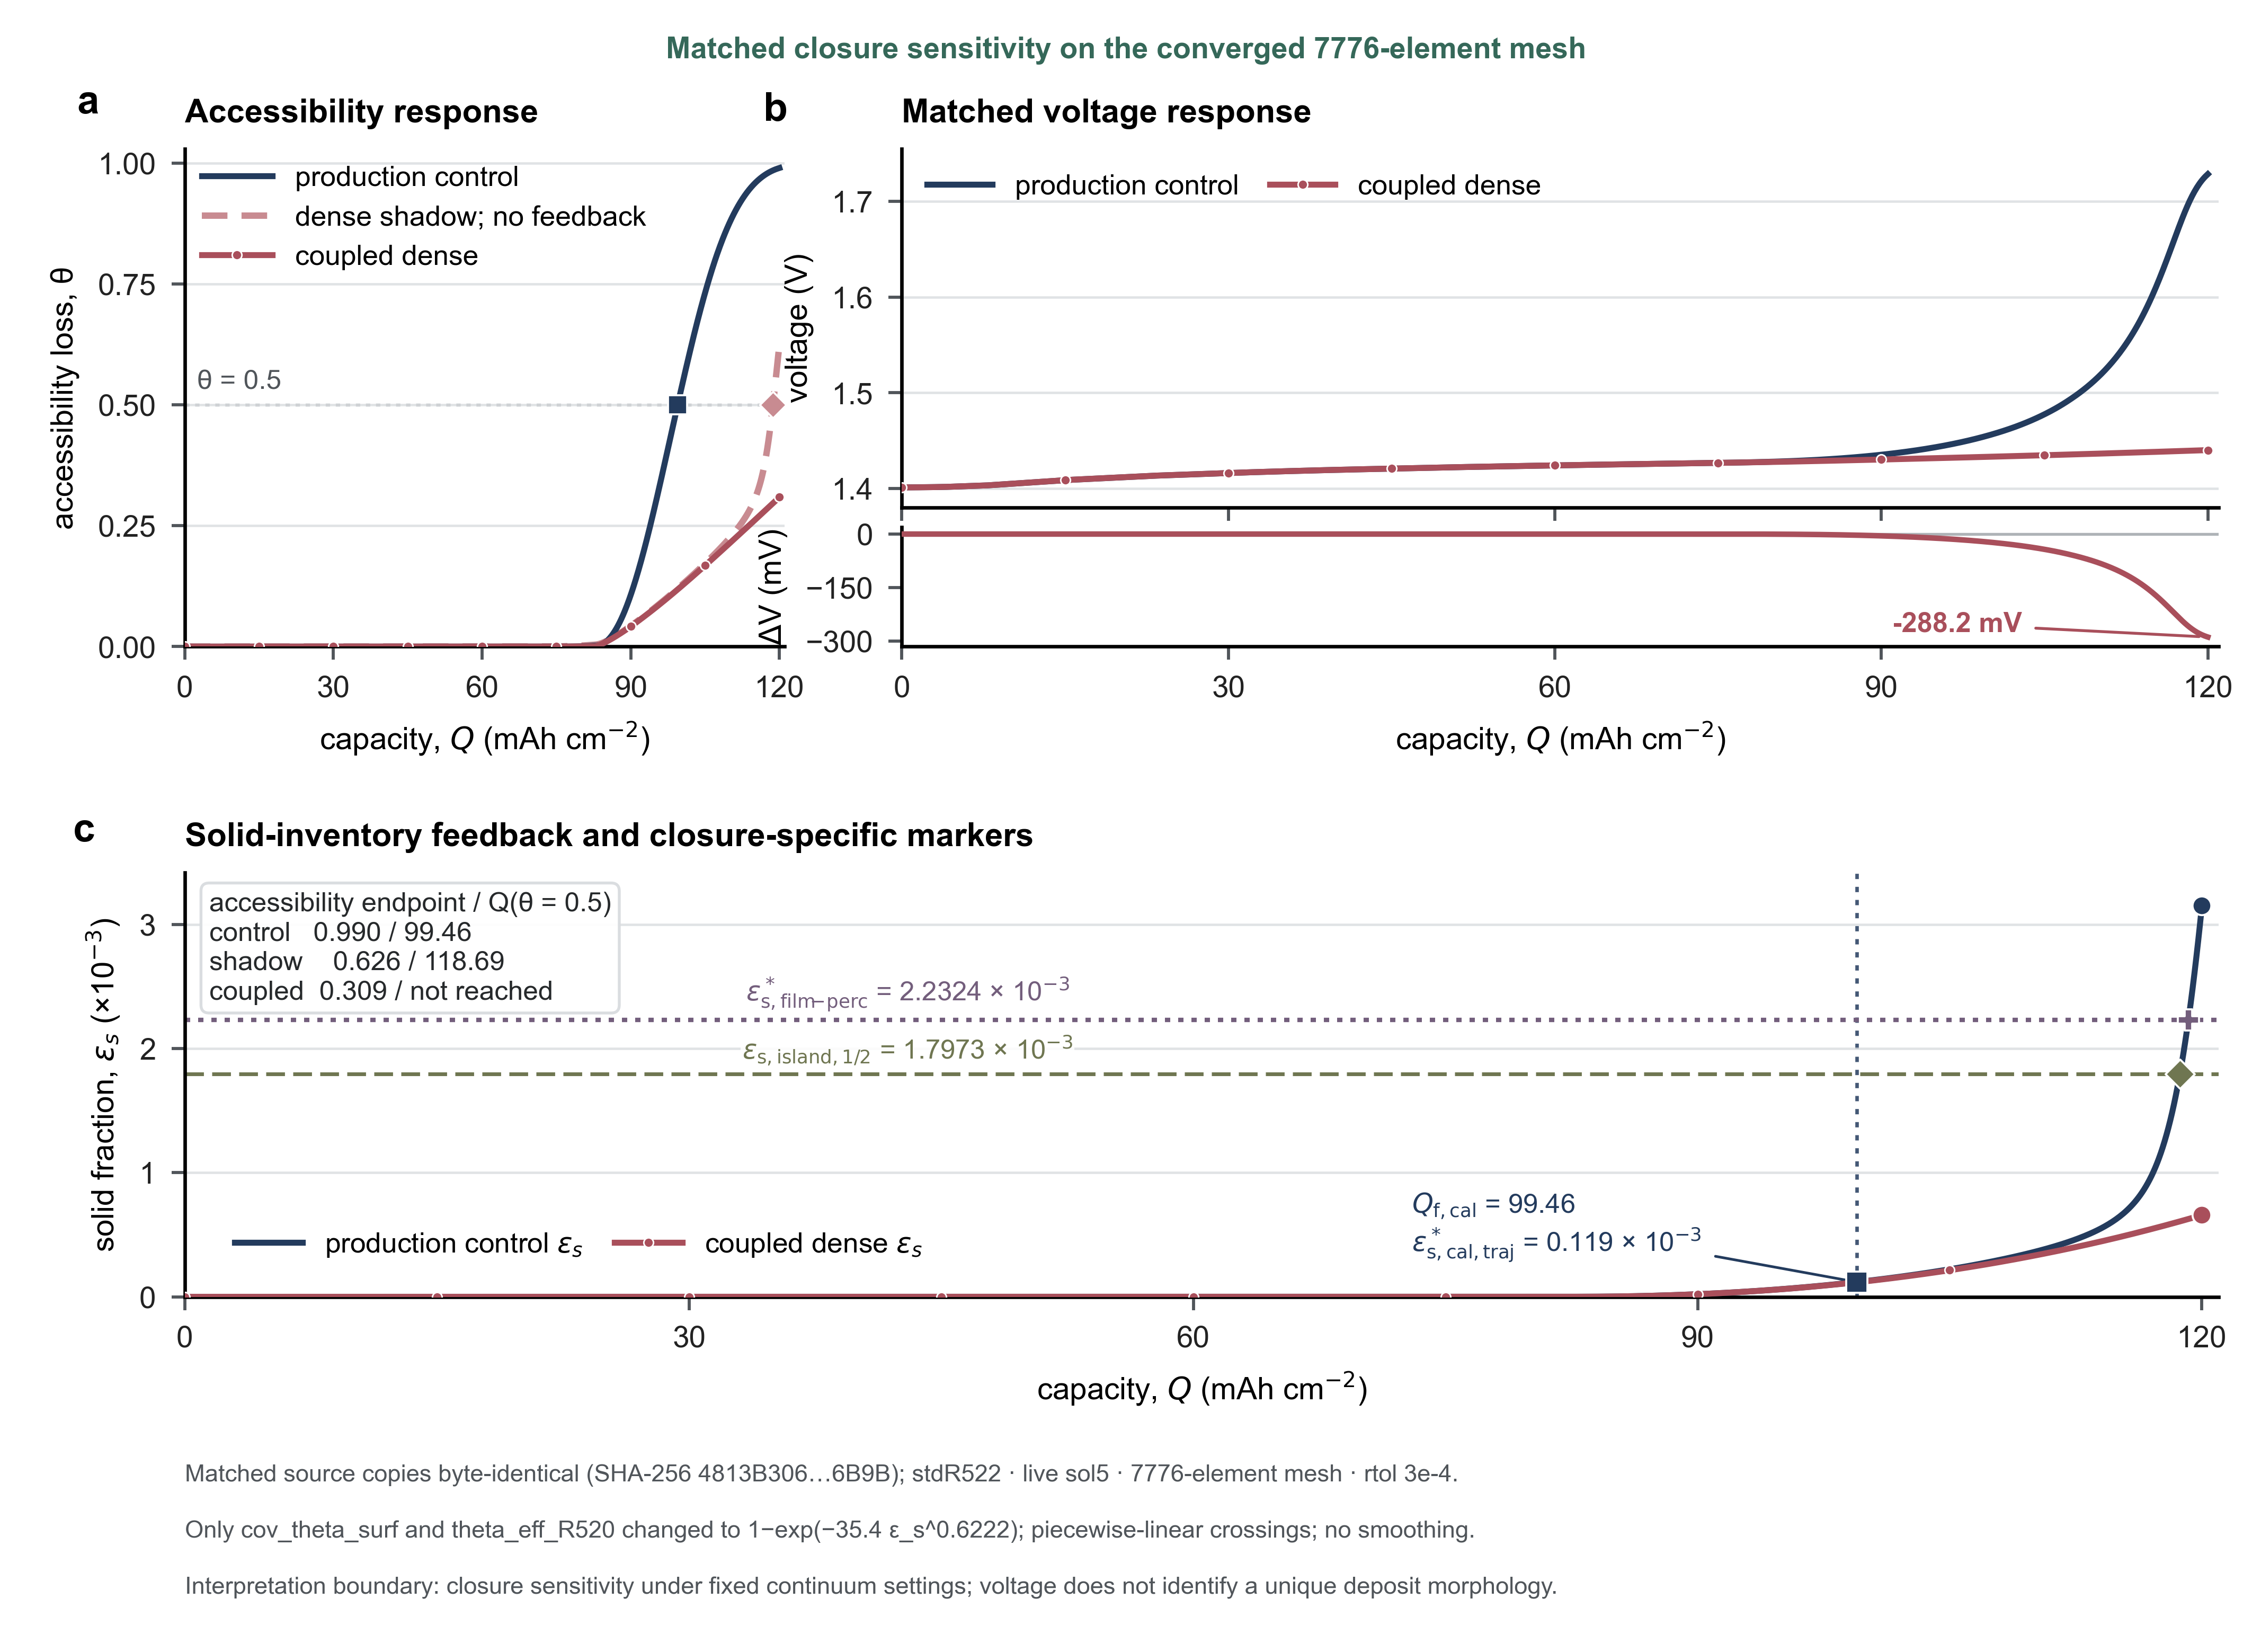
\includegraphics[width=0.98\textwidth]{figures/Fig_R581_matched_closure.pdf}
\caption{\textbf{Matched true-mesh accessibility-closure sensitivity.} (a)~Accessibility loss for the
production control, a one-way dense-island shadow evaluated on the control inventory (no feedback), and the
coupled dense-island solve. (b)~Matched terminal-voltage trajectories and their physical-minus-control
difference. (c)~Each coupled branch's own retained-solid trajectory, with the production-trajectory readout,
dense-island half-accessibility fraction and separate film-percolation comparator kept distinct. The two
7776-element solves used byte-identical source copies, the same study, live solution, time grid and
$\mathrm{rtol}=3\times10^{-4}$; only the two registered accessibility expressions changed. Both the
tighter-tolerance and mesh gates passed. The endpoint difference is $-\SI{288.2}{mV}$, quantifying model-closure
sensitivity rather than identifying a real deposit morphology.}
\label{fig:ablation}
\end{figure}

\subsection{Molecular priors: where iodine is retained and how fast it clears}
\label{sec:res-mol}
The chain begins at the molecular scale, which supplies \emph{bounds and tendencies}---not rate
constants---for two quantities the upper layers inherit. Periodic CP2K places molecular \ce{I2} on the
carbon surface with single-\ce{I2} adsorption energies of $-0.40$ (basal), $-0.85$ (carbonyl, \ce{C=O})
and \SI{-1.00}{eV} (hydroxyl, \ce{C-OH}), and \SI{-0.32}{eV} at a vacancy. Within the registered finite-cell
setup, the more negative oxygen-site values establish only a relative placement ordering. A compact
two-\ce{I2} configuration at \ce{C-OH} is lower in electronic energy by \SI{0.69}{eV} than the registered
separated reference (Fig.~\ref{fig:molecular}a; charge-density-difference maps and projected densities of
states in the SI). Together with independent DFT of iodine on carbon
\citep{Iodine_Graphite_DFT2023,Confinement_JACS2022}, these calculations motivate testing relative siting and
local co-association tendencies only; they do not provide solution free energies, trapping events, a
nucleation pathway, island density $N$, a growth law, or the production accessibility relation. Accordingly,
$N$ is swept as a morphology prior in the physical single-fiber calculations rather than inferred from DFT.
A single-point
cluster diagnostic gives electronic-energy changes of $\SI{-0.46}{eV}$ for the
\ce{I^-}+\ce{I2} cluster and $+\SI{0.05}{eV}$ for the \ce{Br^-}+\ce{I2} cluster
(Fig.~\ref{fig:molecular}b). These are neither solution free energies nor equilibrium constants and do not set
$K_{\mathrm I}$ or $K_{\mathrm{Br}}$; the numerical constants remain conditional literature priors
\citep{Palmer1984,Lee2023}.

Classical molecular dynamics supplies a bulk-electrolyte mobility prior. Under the ECC-scaled parameterization,
the diffusivities of \ce{I^-}, \ce{I3^-} and \ce{I2Br^-} are $1.22$, $0.75$ and
$0.72\times10^{-9}~\si{m^2.s^{-1}}$, respectively (Fig.~\ref{fig:molecular}c). Thus the oxidized carriers are
$38$--$41\%$ slower than iodide within this force-field set. The continuum value
$\Deff=0.5\times10^{-9}~\si{m^2.s^{-1}}$ lies inside the bracket formed by the ECC and formal-charge runs.
Each SOC/charge case contains one \SI{20}{ns} production trajectory. The error bars aggregate four contiguous
time-block stability estimates over the five distinct SOC boxes; they are not independent-replica standard
errors. This is a bounded bulk-electrolyte prior: the MD does not simulate transport through deposited iodine,
validate viscosity or determine an accessibility closure.

\begin{figure}[tbp]\centering
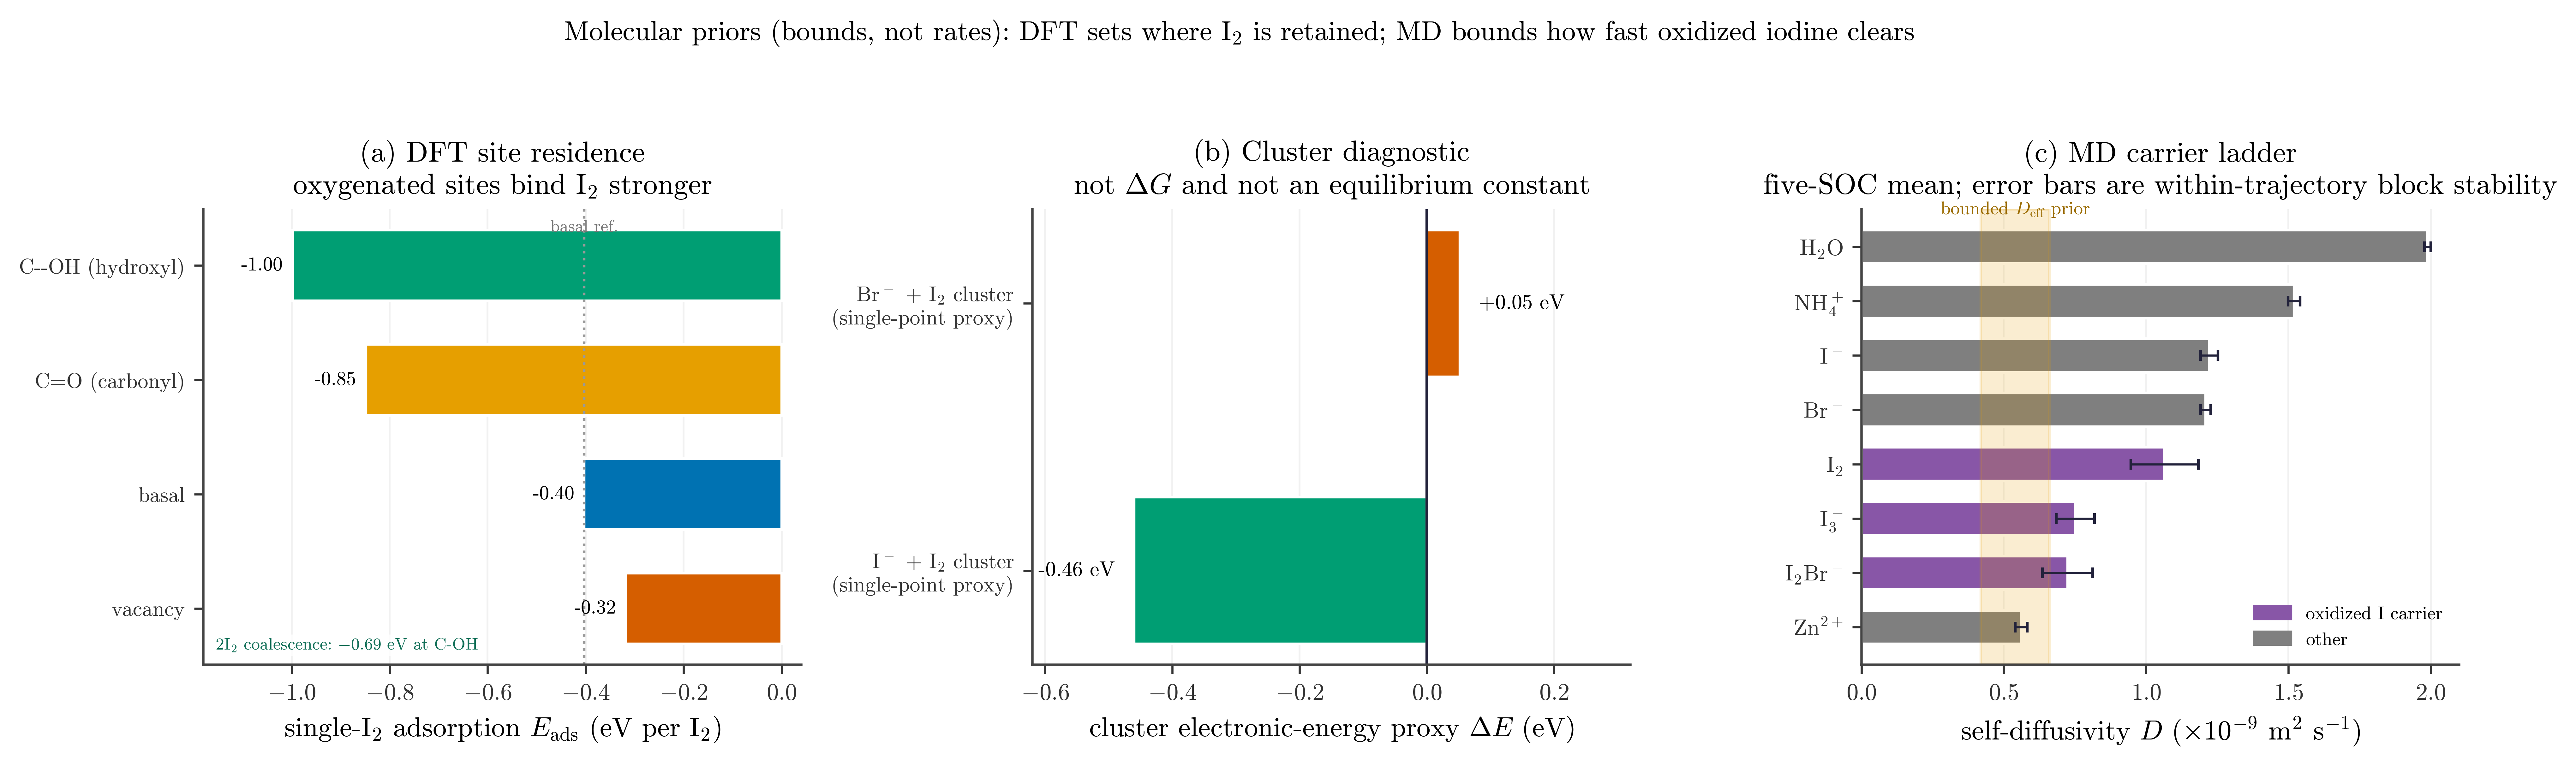
\includegraphics[width=0.99\textwidth]{figures/Fig_R554_molecular_priors.pdf}
\caption{\textbf{Molecular priors (bounds, not rates).} (a) Registered DFT electronic energies establish a
relative single-\ce{I2} site ordering (basal $-0.40$, carbonyl $-0.85$, hydroxyl $-1.00$, vacancy
\SI{-0.32}{eV}) and place a compact 2\ce{I2} configuration at \ce{C-OH} \SI{0.69}{eV} below the registered
separated reference. These finite-cell values are qualitative placement diagnostics, not solution free
energies or nucleation evidence. (b) Single-point cluster electronic-energy diagnostic: values are not $\Delta G$ and do not
determine solution equilibrium constants. (c) MD carrier diffusivities: the oxidized carriers \ce{I3^-} and
\ce{I2Br^-} are $38$--$41\%$ slower than \ce{I^-} (neutral \ce{I2} only $\sim\!12\%$); shaded band is the
low-end $\Deff$ prior. Error bars are propagated four-block within-trajectory stability statistics, not
independent-replica SEM.}
\label{fig:molecular}
\end{figure}

\subsection{Physical mesoscale bounds and matched closure sensitivity}
\label{sec:res-meso}
The single-fiber model supplies a physical isolated-island family, not the magnitude of the production
relation (the geometry is rendered in Supplementary Fig.~\ref{fig:mesomodel}a). For the dense fitted case,
\begin{equation}
\thetaisland=1-\exp\!\left[-35.4\,\varepsilon_{\mathrm{s,reg}}^{0.6222}\right],
\label{eq:theta-island-dense}
\end{equation}
and its half-accessibility fraction is
$\varepsilon_{\mathrm{s,island},1/2}=1.7973\times10^{-3}$. Evaluated one way on the production
$\epss(Q)$ trajectory, the sparse, DFT-clustered, moderate and dense cases end at
$\thetaisland=0.116$, $0.329$, $0.404$ and $0.631$, respectively; the dense shadow projection crosses one
half only at $Q=\SI{118.64}{mAh.cm^{-2}}$. These curves are morphology-prior sweeps with no feedback, and
DFT does not set their $N$ values.

We then performed a fresh matched true-mesh continuum comparison from byte-identical copies of the canonical
input. Both branches use the same study (\texttt{stdR522}), live solution (\texttt{sol5}), 7776-element
mesh, $\mathrm{rtol}=3\times10^{-4}$, output grid and all non-accessibility parameters. The control gives
$Q_{\mathrm s}=82.890$ and $\Qfcal=99.464~\si{mAh.cm^{-2}}$. The coupled dense-island case gives
$Q_{\mathrm s}=82.892~\si{mAh.cm^{-2}}$, but does not reach $\langle\thetaisland\rangle=0.5$ by
$Q=120~\si{mAh.cm^{-2}}$. The endpoint states are
\[
(\langle\epss\rangle,\langle\theta\rangle)_{\mathrm{island}}
=(6.586\times10^{-4},0.309),\qquad
(\langle\epss\rangle,\langle\theta\rangle)_{\mathrm{cal}}
=(3.152\times10^{-3},0.990).
\]
The dense-island terminal voltage is $\SI{288.156}{mV}$ lower. The true-mesh one-way shadow ends at $0.626$
because it uses the control inventory, whereas the coupled case ends at $0.309$ because accessibility feedback
changes the inventory trajectory. Relative to the same-tolerance 1944-element pair, the endpoint voltage
difference changes by only \SI{0.094}{mV}; all predeclared tolerance and mesh gates pass. This registered
comparison quantifies closure sensitivity; it neither validates the production relation nor
identifies an island, film or pore-spanning morphology.
The production-state plots and the $J$--$Q$ map retain the canonical registered values
($Q_{\mathrm s}=83.020$ and $Q_{\mathrm f,cal}=99.590~\si{mAh.cm^{-2}}$); the corresponding true-mesh
control values differ by only $0.130$ and $0.126~\si{mAh.cm^{-2}}$, respectively. Thus, the true-mesh pair
is the authoritative closure-comparison branch, while the frozen canonical branch remains the provenance
anchor for the registered production-state figures.

Three solid-fraction markers are therefore kept separate. The true-mesh production control has
$\langle\epss\rangle=1.190\times10^{-4}$ at $\Qfcal$; the dense physical-island relation reaches one half at
$1.7973\times10^{-3}$; and the separate geometric film-percolation calculation gives
$\varepsilon_{\mathrm{s,film\text{-}perc}}^{*}=2.2324\times10^{-3}$. None is substituted for another.

A pore-throat network (Supplementary Fig.~\ref{fig:mesomodel}b) then tests whether deposited \ce{I2} throttles transport by clogging. For \emph{every}
one of the six deposit-placement laws swept, the network stays $98$--$99\%$ permeable at the operating load
($\epss\sim2$--$4\times10^{-3}$) and the active backbone fully percolates (Fig.~\ref{fig:meso}b). Halving
the permeability requires $30$--$100\times$ the operating load, so a \emph{smooth geometric} permeability
collapse does not drive the calibrated voltage response within the registered smooth-permeability channel.
This rules out only that continuum-permeability
channel: it does not exclude the free-\ce{I2} mass-transfer stress carried in
$\Pi_{\mathrm{gen}}\propto1/\Deff$, viscosity-driven pressure ($\Delta p\propto\mu/K$), or discrete local
pore-throat/shell blockage, which the network does not resolve (Supplementary Table~\ref{tab:channels}). The network does supply one non-continuum constraint a Kozeny--Carman law misses:
blocking efficiency is set by the spatial \emph{overlap} of deposit, not its amount (path-correlated
deposition blocks $\sim\!1.8\times$ more efficiently than surface-spread at the same loading;
Fig.~\ref{fig:meso}c). That deposit placement can matter at fixed inventory is consistent with external
observations: in an analogous flow cell a coalesced passivating layer collapses
efficiency where finely dispersed particles leave the electrode fresh \citep{ZnMnEES2025}, and the
accessibility of a retained halogen phase is governed by its physical state \citep{XuZnBr2024}. In a
non-iodine TEMPO/\ce{KBF4} flow-cell analogue, operando neutron imaging linked unintended salt precipitation
to obstructed ion transport and reduced available surface area \citep{RFB_SEF2025}. The present model keeps these physical
bounds separate from the voltage-calibrated production relation.

How each closure enters the model also tells us what it is sensitive to. The selected accessibility relation feeds the
continuum kinetics through the accessible-area prefactor $(1-\theta)$, and hence the charge-voltage
response, whereas the relative permeability $K(\epss)$ feeds only the Darcy flow. Because $K$ is a
\emph{geometric} closure, these two transport channels respond to different electrolyte properties and do not
mix: the free-\ce{I2} generation load scales as $\Pi_{\mathrm{gen}}\propto1/\Deff$, so it tracks the
oxidized-carrier diffusivity, while the hydraulic pressure across the felt scales as $\Delta p\propto\mu/K$,
so it tracks the viscosity. A more viscous electrolyte therefore raises pumping pressure without directly
moving the averaged-saturation marker, whereas a slower-diffusing one raises $\Pi_{\mathrm{gen}}$ and brings
that marker forward (Supplementary Table~\ref{tab:channels}). The modular closures make this separation explicit, and it gives
a change of supporting electrolyte a quantitative route into the model. The pore network therefore bounds
only the \emph{smooth geometric} permeability channel of panel~(b); the mass-transfer and viscosity channels
of panels~(c,d) are separate and remain active, which is why a change of electrolyte that alters diffusivity
or viscosity moves the operating point even when the geometric $K(\epss)$ barely does.

\begin{figure}[tbp]\centering
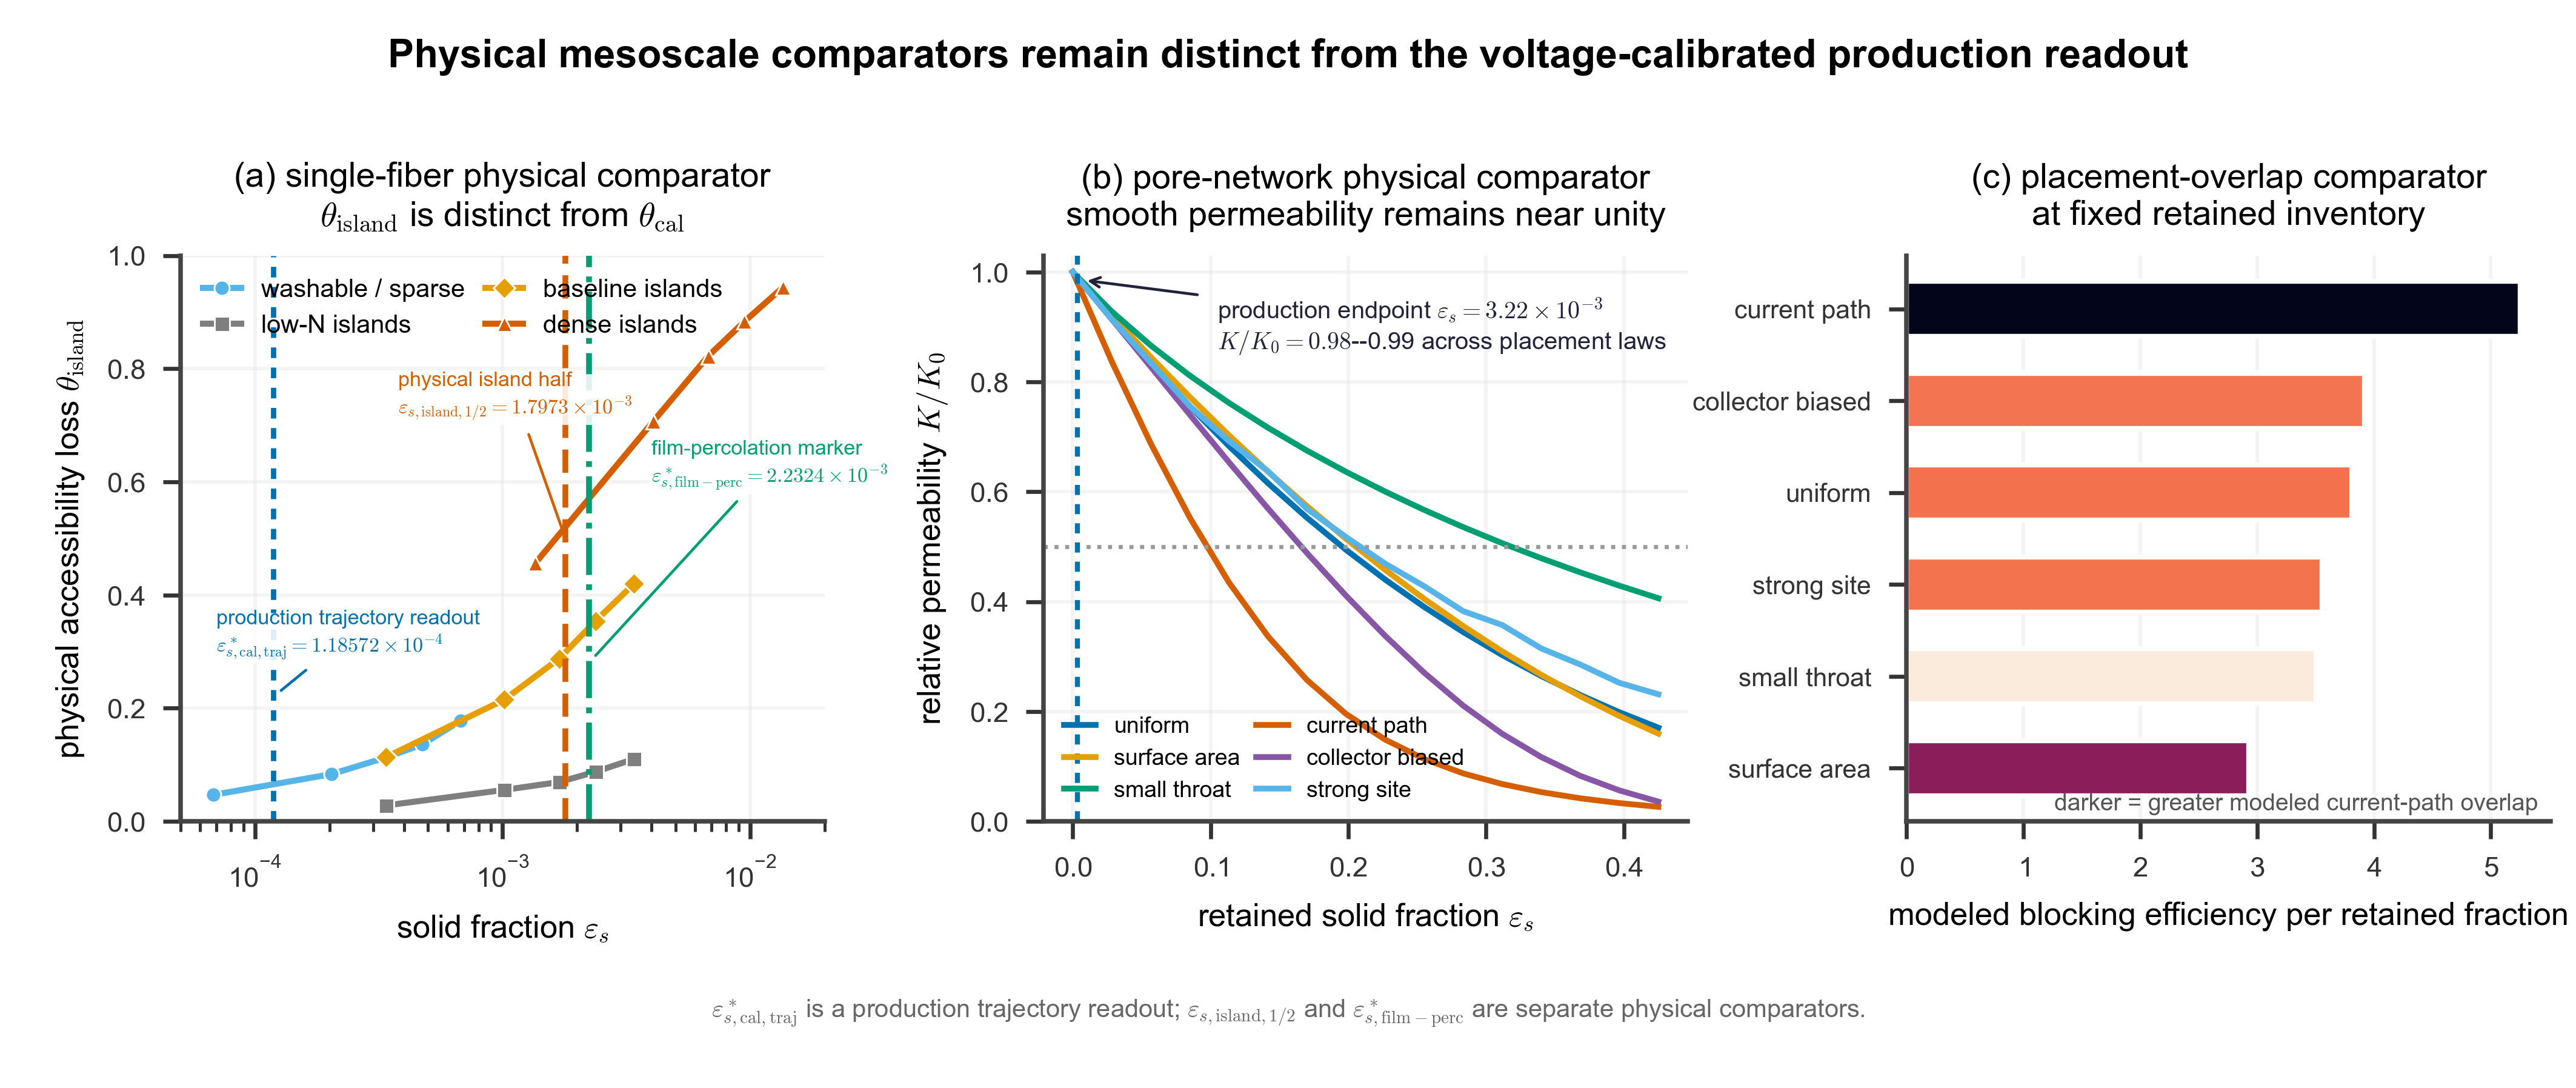
\includegraphics[width=0.99\textwidth]{figures/Fig_R555_mesoscale_closures.pdf}
\caption{\textbf{Physical bounds from the mesoscale models.} (a) Physical isolated-island accessibility
$\thetaisland(\epss)$ for the tested morphology families; the dense fitted half-accessibility fraction is
$\varepsilon_{\mathrm{s,island},1/2}=1.7973\times10^{-3}$. (b) Pore-network smooth relative permeability
remains near unity over the modeled operating load and halves only at much larger solid fractions.
(c) At fixed solid inventory, blocking efficiency depends on deposit placement. The separate geometric
film-percolation marker is $\varepsilon_{\mathrm{s,film\text{-}perc}}^{*}=2.2324\times10^{-3}$. These physical
bounds do not determine the production voltage-calibrated accessibility magnitude.}
\label{fig:meso}
\end{figure}

\subsection{The transport and formulation envelope}
\label{sec:res-sens}
The operating boundary is controlled by a small set of transport and formulation levers, and we now map how
much each one moves it. Two of them, the intrinsic dilute-water reference $\csat$ (and therefore
$\csat^{\mathrm{eff}}$ at fixed $\gamma_{\mathrm{salt}}$) and the rate-closure efficiency
$\phi_{\mathrm{ppt}}$, enter the reduced criterion algebraically rather than by re-solving the transport.
Their leverage is therefore swept as a postprocess on the baseline trajectory, exact with respect to the
reduced criterion, though not a re-solved full cell. Raising $\csat$ delays the averaged-saturation marker
strongly: it moves from $Q_{\mathrm s}=65$ to $\SI{109}{\mAhcm}$ as $\csat$ rises from $1.0$ to
$2.0~\si{mol.m^{-3}}$. At $\csat=\SI{2}{mol.m^{-3}}$ the marker reaches the window edge and the production
half-accessibility marker is not reached; above it the registered averaged saturation crossing is absent
($S_{\max}<1$). Propagated as an uncertainty rather than a lever, the literature spread
of the aqueous solubility maps the baseline marker onto an explicit error band for the least-constrained
constant: $Q_{\mathrm s}\approx71$ at $\SI{1.1}{mM}$, $\approx76$ at $\SI{1.2}{mM}$, and $83$ at the adopted
$\SI{1.33}{mM}$. The rate-closure efficiency $\phi_{\mathrm{ppt}}$ sets the width of the
modeled interval: lowering $\phi_{\mathrm{ppt}}$ leaves the saturation marker $Q_{\mathrm s}$ fixed
but pushes $\Qfcal$ outward, widening $\Delta Q_{\mathrm{cal}}$ from $17$ to
$\SI{29}{\mAhcm}$. The diffusivity channel is a seven-point \emph{solved}
COMSOL sweep: the saturation marker rises smoothly from $Q_{\mathrm s}=45$ to
$\SI{106}{\mAhcm}$ as $\Deff/D_0$ goes from $0.5$ to $2$, following $\Pi_{\mathrm{gen}}\propto1/\Deff$.
Because the mass-transfer stress depends only on the combination $\delta/\Deff$, the boundary-layer
thickness and the diffusivity collapse onto one axis: both production markers slide together as $\delta/\Deff$
varies. The free-\ce{I2} generation stress, not $\csat$ alone, therefore remains
central to this marker. The hydraulic consequence is separate again: viscosity multiplies the pressure drop
directly, $\Delta p/\Delta p_0=(\mu/\mu_0)/(K/K_0)$, and is a formulation input rather than a quantity hidden
inside the geometric permeability $K(\epss)$. Ranking every lever by the fractional shift of its primary
model coordinate then answers which uncertainty actually
moves the boundary: over the tested ranges the transport group ($\delta/\Deff$, $\Deff$) produces the largest
saturation-marker span, the solubility reference follows, and the production accessibility-closure parameters
move $\Qfcal$;
viscosity is the largest \emph{pressure} lever, while the smooth $K(\epss)$ response is negligible over the
modeled load. Together these sweeps turn the scope bounds (scope-and-bounds table in the SI)
into quantified sensitivities rather than asserted caveats. Full per-family values and evidence classes are
reported in the Supplementary Information.

\subsection{A conditional operating map and external dissolution scales}
\label{sec:res-rate}
The iodine-state progression projects into an operating boundary in the current-density/areal-capacity plane
(Fig.~\ref{fig:jqmap}). Both the saturation boundary, $J_s^{+}(Q)$, and the production half-accessibility
boundary, $J_{b,\mathrm{cal}}^{+}(Q)$, are conditional on the registered parameterization. Converged marker
solves at $J=20$ and $40~\si{mA.cm^{-2}}$ anchor the local interpolation. The registered $J=40$ trajectory
also supplies $\Qfcal$. No physical-island failure boundary is inferred.

\begin{figure}[tbp]\centering
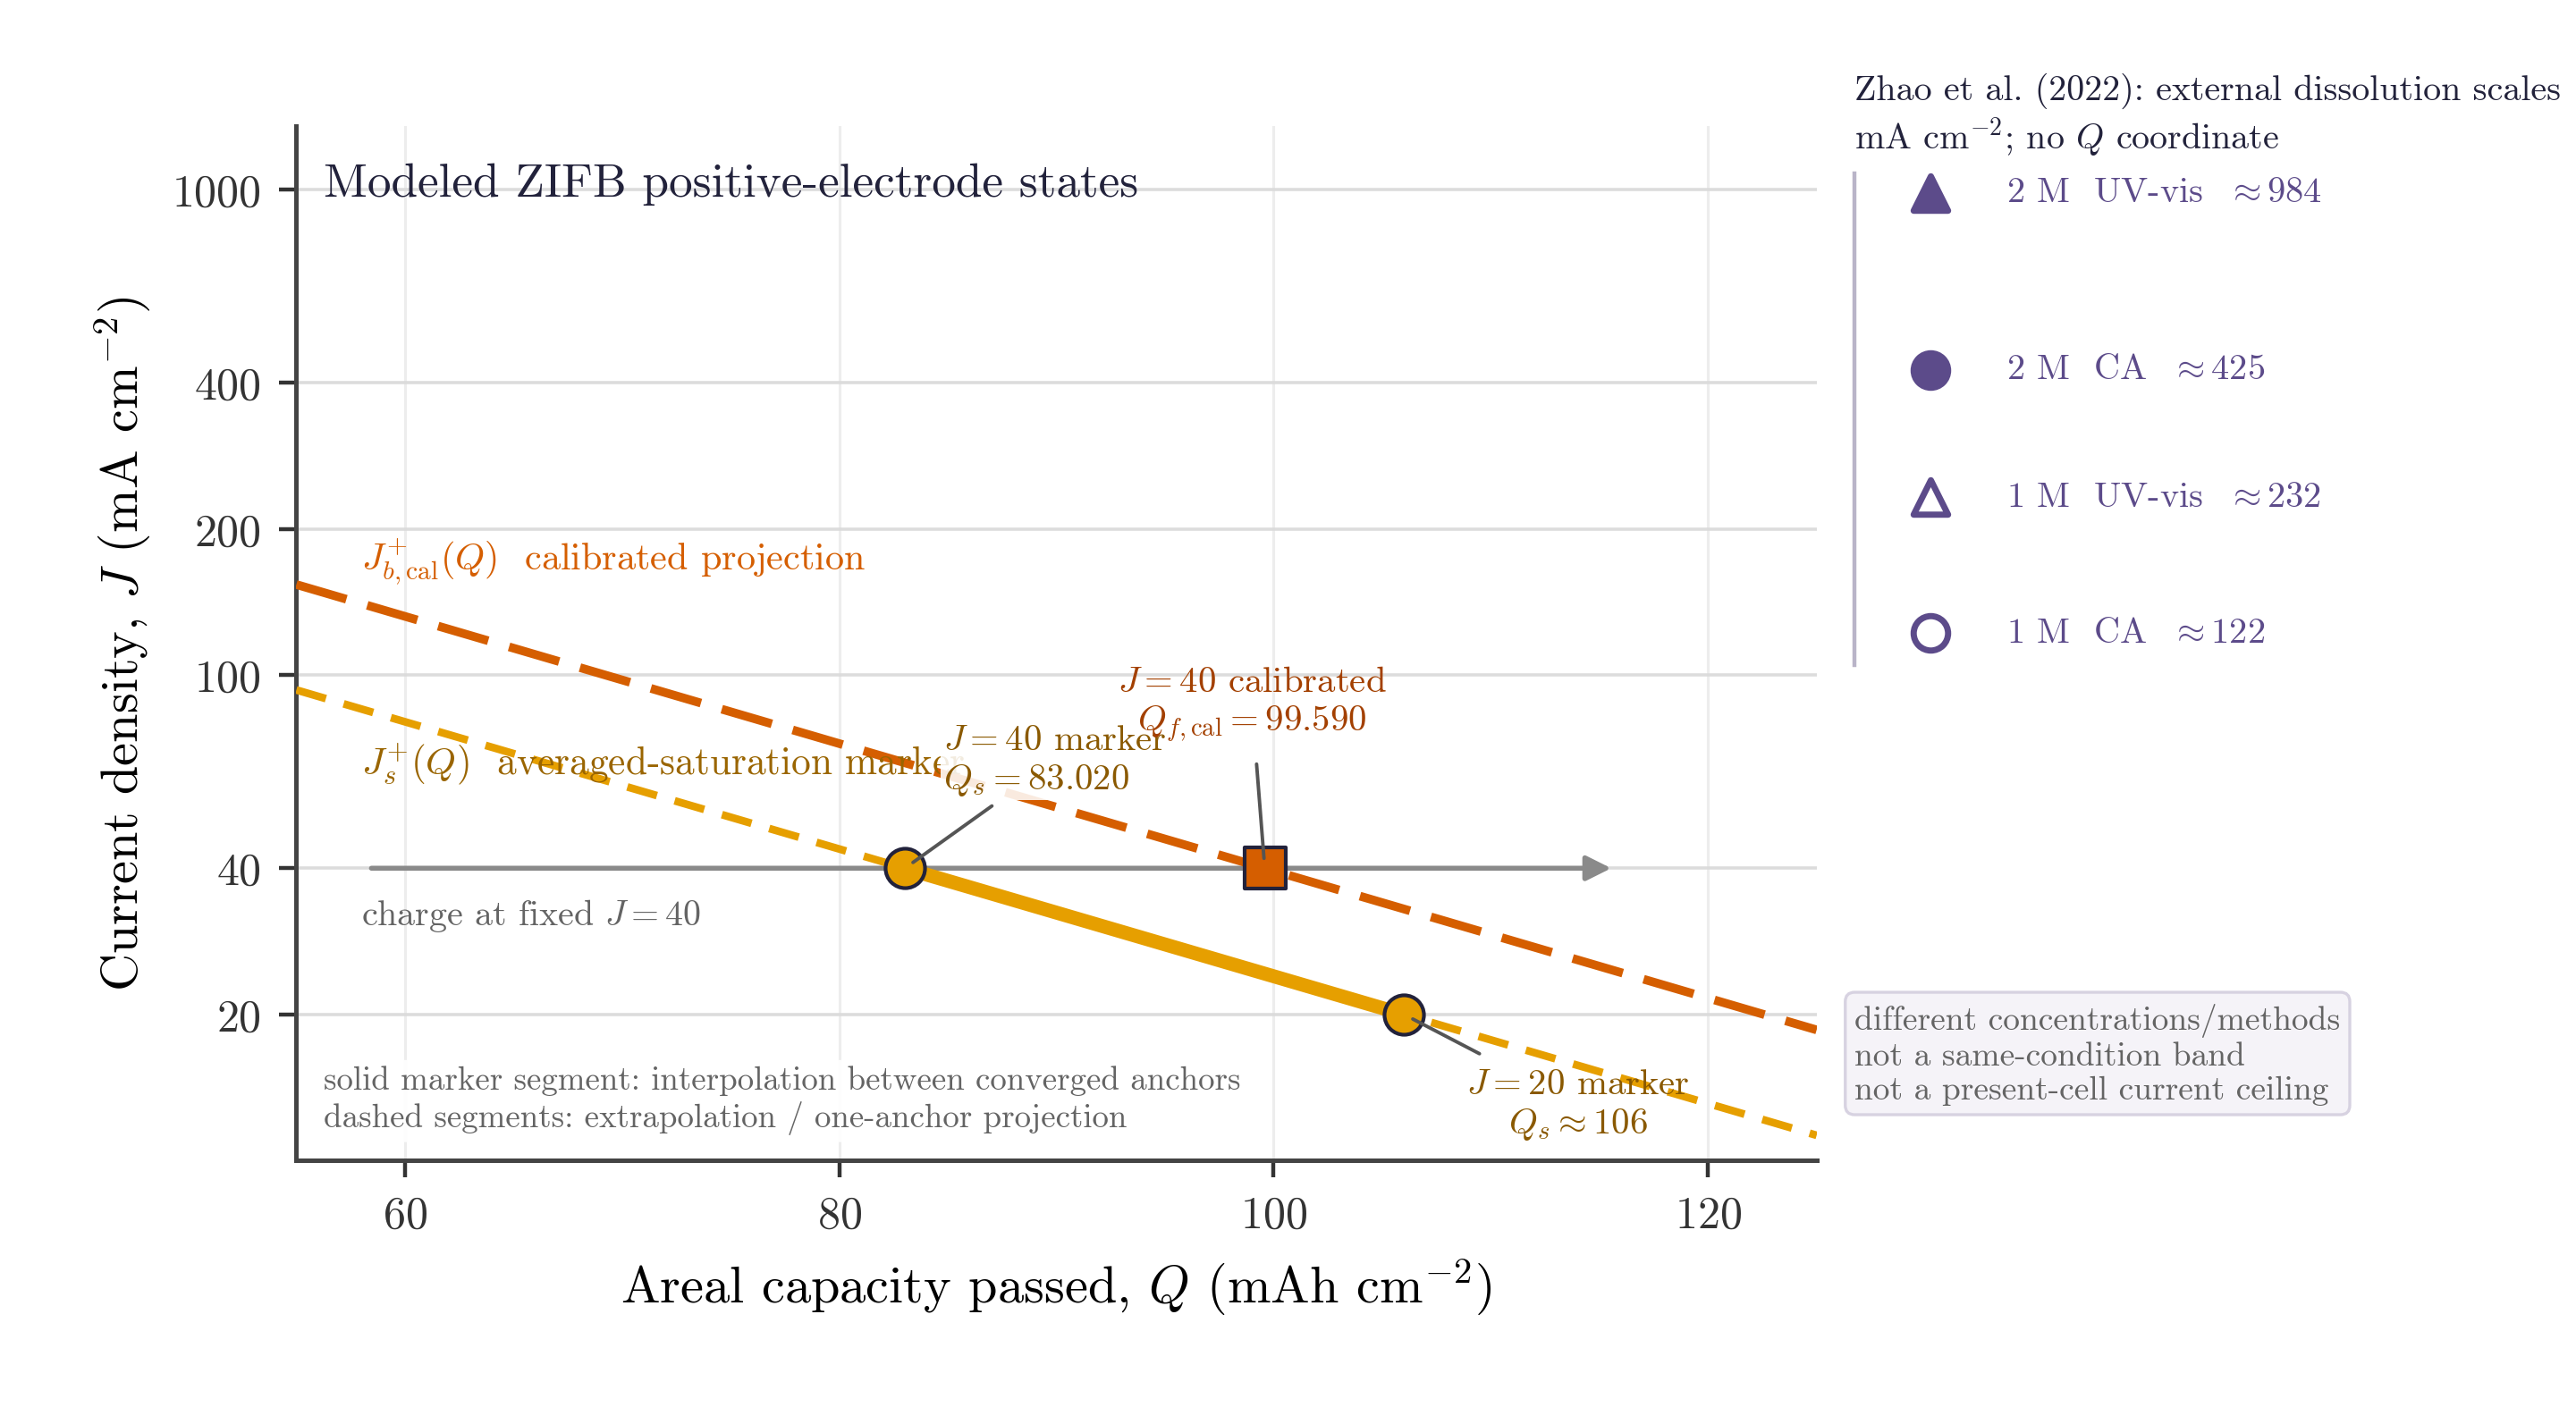
\includegraphics[width=\textwidth]{figures/Fig_R581_jq_map.pdf}
\caption{\textbf{Organizing map for the modeled ZIFB positive-electrode states.}
At fixed current, increasing $Q$ crosses the modeled saturation boundary $J_s^+(Q)$ and, on the production
closure, the calibrated half-accessibility projection $J_{b,\mathrm{cal}}^+(Q)$. Circles are converged
saturation-marker
solves at $J=20$ and $40~\si{mA.cm^{-2}}$; the square is the registered $J=40$ marker
$\Qfcal=\SI{99.590}{mAh.cm^{-2}}$. The solid saturation-marker segment is the interpolation between the two
converged anchors. Dashed saturation-marker segments are extrapolations, and the dashed
$J_{b,\mathrm{cal}}^+$ curve is a parallel
one-anchor projection rather than a solved boundary. The separate right-hand rail
lists the four concentration- and method-specific dissolution-derived scales reported by Zhao \emph{et al.}
\citep{Zhao2022}; the rail has no $Q$ coordinate and is neither a same-condition band nor a current ceiling for
the present cell. Source data are provided with the figure package.}
\label{fig:jqmap}
\end{figure}

The map carries conditional model magnitudes and external kinetic context; it does not turn them into one
validated ceiling. Published iodine-dissolution measurements provide an external kinetic scale rather than a
calibrated ceiling for the present electrolyte. Zhao \emph{et al.} reported method-dependent fluxes
corresponding to approximately $122$ (chronoamperometry) and $232~\si{mA.cm^{-2}}$ (UV--visible) at
\SI{1}{M} iodide, and $425$ (chronoamperometry) and $984~\si{mA.cm^{-2}}$ (UV--visible) at \SI{2}{M}
iodide \citep{Zhao2022}. The former $232$--$425~\si{mA.cm^{-2}}$ span combined different concentrations and
methods and is not retained as a same-condition band. These values motivate a clearance-versus-generation
hypothesis but do not independently validate a sustainable charge-current ceiling for the present
\ce{ZnI2}/\ce{NH4Br} cell. Likewise, the charge-side production marker and measured maximum discharge
capacities are different observables and are not equated.

\paragraph{Literature anchors for the clearance hypothesis.}\label{sec:rate}
The relation $i^{*}=2Fk$ translates reported heterogeneous \ce{I2}-dissolution fluxes into a
condition-labelled current scale; it is not fitted to the present cells. Accelerating dissolution with a
cosolvent increases that scale \citep{Zhao2022}. Independent literature also supports positive-electrode
accessibility and kinetic penalties in iodine-precipitation regimes: a
dense \ce{I2} film raises the positive charge-transfer resistance roughly ninefold
($16.5\!\to\!147.4~\si{\ohm.cm^2}$) \citep{Jang2021}, and positive-electrode catalysts or accelerated iodine
dissolution can improve high-rate behavior \citep{ShakeriHosseinabad2023,Yang2023}. These examples are
mechanistic context, not validation of a common ceiling or of the present thresholds.

\paragraph{Representative supporting-electrolyte context.}\label{sec:res-chem}
The positive-electrode scaffold is evaluated at a representative
\SI{1}{M}~\ce{ZnI2}$+$\SI{4}{M}~\ce{NH4Br} condition. In the rebuilt common-current full-cell series, the
maximum of the within-command-level median delivered capacity increased descriptively from
$40.84~\si{mAh.cm^{-2}}$ at 0 M to $137.54~\si{mAh.cm^{-2}}$ at 4 M NH4Br. Independent-cell counts were
$1/1/1/2/1$ for 0/1/2/3/4 M, respectively. This protocol-bounded association neither establishes a population
fold change or saturation law nor validates the continuum thresholds. The complete composition trajectories,
selection rules and endpoint sensitivities are reported in the Supplementary Information. NH4Br is retained
here only as the representative supporting electrolyte; the paper's mechanistic claims concern the ZIFB
positive electrode.

\subsection{Bounding the alternative failure channels}
\label{sec:perm}
We bound two alternatives rather than excluding all transport or film mechanisms. \emph{Not a smooth
geometric permeability collapse}: the
relative permeability stays near unity throughout (Kozeny--Carman endpoint $0.96$, pore-network $0.98$;
$K/K_0=0.998$ at $\langle\thetacal\rangle{=}\tfrac12$ on the production trajectory), so injecting the physical pore-network closure in place of the
mean-field one shifts the cell voltage by only \SI{1.27}{mV} (permeability-injection figure in the SI). The full two-way
Darcy flow is likewise immaterial to the solved saturation marker (with the $\delta$ sub-grid caveat of
\S\ref{sec:knob-mechanism}): the solved velocity field is nearly invariant ($<\!0.1\%$ over a charge), and a
separate frozen-velocity control leaves the registered saturation marker unchanged. This isolates the
\emph{geometric} permeability channel and does not remove transport from
the mechanism: the free-\ce{I2} generation stress $\Pi_{\mathrm{gen}}=\iapp\delta/(2F\Deff\csat)$ remains
central to the super-saturation marker. Discrete local pore-throat/shell blockage and viscosity-driven
pressure ($\Delta p\propto\mu/K$) lie outside what the near-unity geometric $K(\epss)$ tests
(Supplementary Table~\ref{tab:channels}). Within the registered production parameterization, the modeled
failure coordinate is loss of \emph{accessible reaction sites}, not a smooth geometric permeability collapse.
The far-extrapolated hydraulic response as $K/K_0\!\to\!0$ is a distinct downstream scenario outside the
validated range and present scope. \emph{Voltage is morphology-non-identifying}:
the terminal voltage does not uniquely identify deposit morphology. In the reduced observation layer,
accessibility loss and the Tafel-like coefficient trade off over a broad range, so the same voltage trend can
be represented by different effective accessibility states. The physical isolated-island shadow calculations
bound one geometric response, while the production relation is an effective voltage-calibrated response. In
the registered matched solves, replacing only the accessibility relation changes the terminal voltage by
$-\SI{288.156}{mV}$ and changes the coupled solid-inventory trajectory (\S\ref{sec:res-meso}). Their difference
shows model-form sensitivity, not proof of a coalesced film. The current evidence therefore supports only the
following statement: under the fixed production parameterization, a stronger effective accessibility-loss
response than the tested isolated-island relation is needed to reproduce the calibrated late-rise branch, but
the responsible morphology remains unresolved. The smooth bulk-permeability calculation rules out only a
mean-field hydraulic collapse over the modeled load and does not decide among local pore-throat, shell,
island-coalescence or other accessibility-loss mechanisms. As external context, a dense iodine film has been
reported to raise positive-electrode charge-transfer resistance approximately ninefold \citep{Jang2021}; a
uniform area-blocking translation would correspond to an effective accessibility loss near $0.89$, but this
mapping is not a morphology measurement for the present cell.

Beyond these internal alternatives, three \emph{external} channels can also close a ZIFB operating window, and
the present mechanism is bounded against each rather than claimed to supersede them. First, the negative
zinc electrode: two ZIFB degradation studies attribute their reported performance limit to a dense zinc layer or dendrite
front at the anode \citep{Richtr2026,ChaNatCommun2025}. Those reports identify negative-side degradation in
their cells; this is complementary to, but does not exclude, positive-side limitations under other operating
conditions (\S\ref{sec:scope}). Second, altered speciation or
storage pathways: quaternary-ammonium chemistry can form an insoluble iodine-containing salt, while halide
mediation can redirect oxidized-iodine speciation \citep{JiangQA2024,Liao2025}; neither regime is represented
by the present unmediated \ce{I2}/\ce{I^-} branch. Third, adsorptive site passivation on catalytic
hosts can dominate on strongly binding carbons \citep{Xiao_JACS2025}; the felt-class carbon modeled here
carries no such catalyst. Each competing channel therefore sharpens, rather than contradicts, the scope of the
saturation--deposition--accessibility positive-electrode scaffold.

\subsection{Operating and design levers act on three nodes}
\label{sec:knob-mechanism}
Every global operating variable examined here acts on one of the terms in
$S_{\mathrm{base}}=\gamma_{\mathrm{salt}}(\Pi_{\mathrm{inv}}+\Pi_{\mathrm{gen}})/\beta_{\mathrm{intra}}$
(\S\ref{sec:theory}): the
free-\ce{I2} generation stress $\Pi_{\mathrm{gen}}=\iapp\delta/(2F\Deff\csat)$ is moved by rate, the
oxidized-carrier diffusivity, mechanical compression and the intrinsic reference $\csat$ (through
$\csat^{\mathrm{eff}}$ at fixed $\gamma_{\mathrm{salt}}$); the
retained-inventory stress $\Pi_{\mathrm{inv}}=c_{\mathrm{I_2,tot}}/\csat$ by the state of charge; and the
within-cycle buffer $\beta_{\mathrm{intra}}$ by the supporting electrolyte. Conductivity, by contrast, moves
the cell voltage but leaves the saturation marker pinned, a clean negative control. The solved
flow rate also leaves that marker pinned, but partly \emph{by construction}: the fiber-scale boundary layer
$\delta$ that carries the mass-transfer stress is a sub-grid parameter decoupled from the electrode-scale
Darcy field, so the solve does not capture the physical route by which a higher flow rate thins $\delta$ and
lowers $\Pi_{\mathrm{gen}}$. That route is instead quantified analytically by the $\delta/\Deff$ sweep in the
Supplementary Information. Ranking every lever
by the node it perturbs and its effect on $S$ places the oxidized-carrier diffusivity as the dominant lever
through $\Pi_{\mathrm{gen}}\propto1/\Deff$ (Table~\ref{tab:knobs}; the per-family COMSOL scans and a
phase-plane view, in which each lever is a distinct move on one saturation boundary, are in the Supplementary
Information).

\begin{table*}[t]\centering\small
\caption{\textbf{Model-internal operating and design levers for the ZIFB positive electrode.}
Each row states the model channel, directional response and evidence class. Numerical sweep details are given
in the Supplementary Information.}
\label{tab:knobs}
\begin{tabular}{@{}p{3.0cm} p{3.5cm} p{6.2cm} p{2.2cm}@{}}
\toprule
Knob / family & Model channel & Directional response & Evidence class\\
\midrule
Oxidized-carrier diffusivity & $\Pi_{\mathrm{gen}}\propto1/\Deff$ & Lower $\Deff$ advances $Q_{\mathrm s}$ and increases the production solid/accessibility response. & bounded MD prior; solved sweep\\[2pt]
Apparent iodine solubility & $\Pi_{\mathrm{inv}},\Pi_{\mathrm{gen}}\propto1/\csat$ & Lower $\csat$ reduces headroom on both stress terms and advances $Q_{\mathrm s}$. & bounded literature prior\\[2pt]
Applied current density & $\Pi_{\mathrm{gen}}\propto\iapp$ & Higher current raises the generation stress and advances modeled saturation. & solved points plus interpolation\\[2pt]
Mechanical compression & $\epsl L$ and $\Deff$ & Compression changes pore inventory and transport; the available cells test direction only. & solved model; descriptive data\\[2pt]
Charge passed / iodine inventory & $\Pi_{\mathrm{inv}}(Q)$ & Charging increases inventory stress along the registered trajectory. & solved state coordinate\\[2pt]
Representative supporting electrolyte & $\beta_{\mathrm{intra}}$ and unsolved transport/speciation inputs & NH4Br sets the baseline condition; cross-composition effects are not separated. & prescribed baseline; descriptive data\\[2pt]
Wetted area $a_s$ & local current distribution, not global $\Pi_{\mathrm{gen}}$ & One branch changed current crowding; the sign is not identified. & one branch only\\[2pt]
Conductivity and flow & voltage / boundary-layer channels & Conductivity changes voltage without moving $S$; flow acts through unresolved $\delta(v)$ in the reduction. & control and analytic bound\\
\bottomrule
\end{tabular}
\end{table*}

Three tiers emerge (Table~\ref{tab:knobs}). The largest raw effects, the oxidized-carrier diffusivity prior and
the salting-out solubility, set the absolute failure scale but rest on the least-constrained inputs, so their
\emph{ranking}, not any calibrated magnitude, is load-bearing. The leading operationally accessible, clean
lever is the applied current density. Conductivity forms an orthogonal voltage channel that leaves
the saturation marker pinned (the clean negative control). The solved flow also leaves that marker pinned;
because the fibre boundary layer $\delta$ is sub-grid, we test this analytically with a flow-dependent
$\delta(v)$ scenario from a Sherwood correlation ($Sh=a\,Re^{m}Sc^{1/3}$, $\delta\propto v^{-m}$;
Fig.~\ref{fig:flowdelta}): across the operating range $25$--$\SI{100}{mL.min^{-1}}$ the marker moves only
$\approx\SI{11}{\mAhcm}$ (Sherwood exponent $m=0.4$--$0.6$), against $\approx\SI{61}{\mAhcm}$ for the
$\Deff$ and rate levers, so flow remains the weaker saturation-marker lever within this declared
boundary-layer scenario.
These model trends are juxtaposed with descriptive, single-cell compression capacity brackets in the SI;
those measurements do not independently validate the modeled trend.

\begin{figure}[tbp]\centering
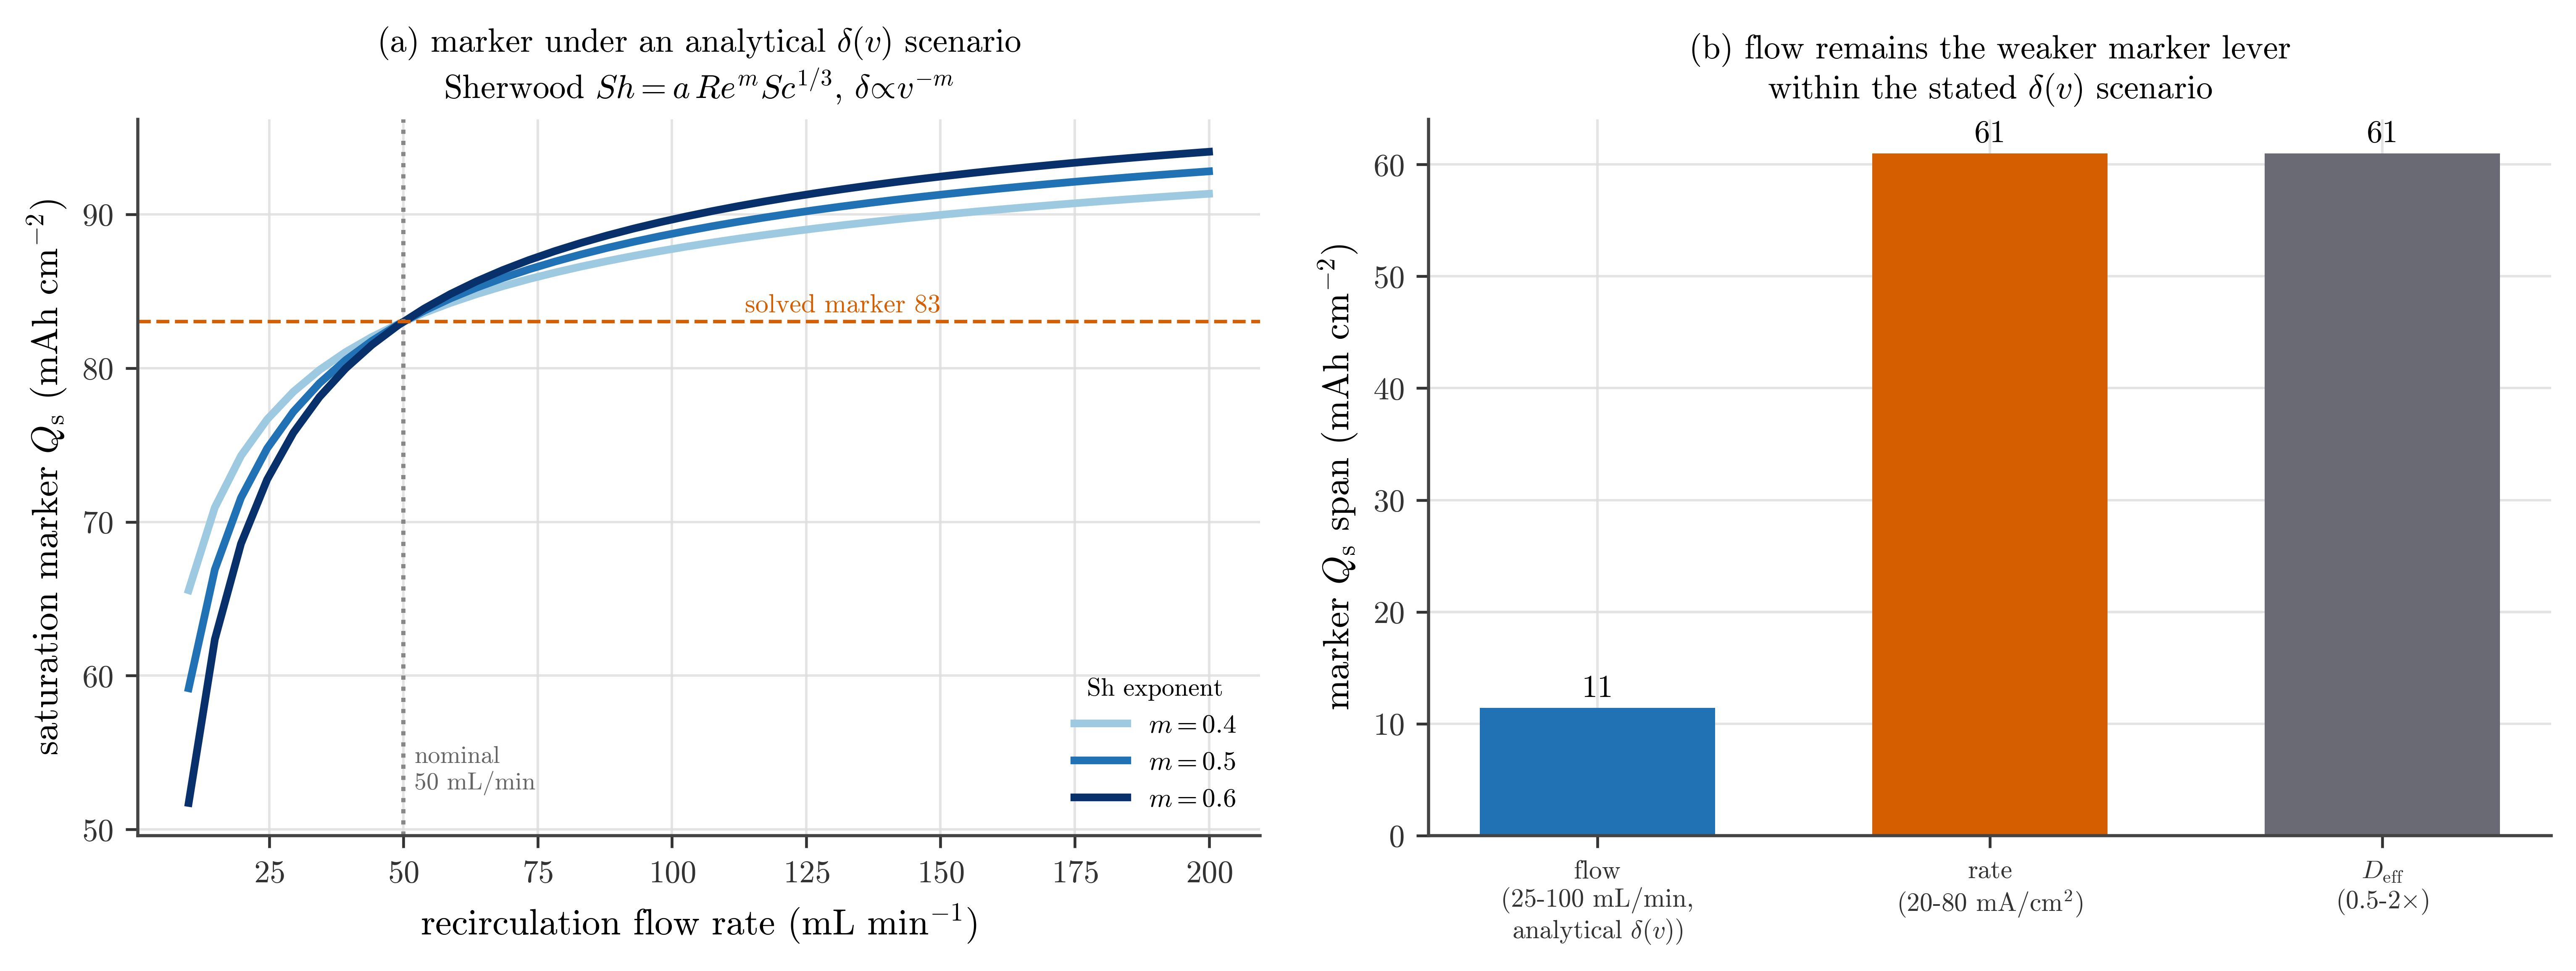
\includegraphics[width=0.92\textwidth]{figures/Fig_R577_flow_delta.pdf}
\caption{\textbf{Flow remains a weak saturation-marker lever in an analytical boundary-layer scenario.} The
solved Darcy flow leaves the marker pinned partly because the fibre Nernst layer $\delta$ is a sub-grid parameter;
here $\delta$ is made flow-dependent through a Sherwood correlation ($Sh=a\,Re^{m}Sc^{1/3}$, so
$\delta\propto v^{-m}$), anchored to $\delta=\SI{25}{\micro m}$ at the nominal \SI{50}{mL.min^{-1}}, and only
the generation stress $\Pi_{\mathrm{gen}}$ scales with flow while $\Pi_{\mathrm{inv}}(Q)$ and $\beta(Q)$ are
read from the solved baseline. (a)~Saturation marker $Q_{\mathrm s}$ versus recirculation rate for Sherwood
exponents $m=0.4$--$0.6$. (b)~Over the operating range $25$--$\SI{100}{mL.min^{-1}}$ the marker shifts by only
$\approx\SI{11}{\mAhcm}$, against $\approx\SI{61}{\mAhcm}$ for the $\Deff$ and rate levers. This declared
correlation bounds, but does not measure, the unresolved sub-grid $\delta(v)$ channel.}
\label{fig:flowdelta}
\end{figure}

\paragraph{Design implication.} The registered production branch places its saturation and calibrated
half-accessibility markers at $83.0$ and $99.6~\si{mAh.cm^{-2}}$, respectively. These conditional model
coordinates are used to compare lever directions, not as demonstrated electrode limits.
Operationally, halving
the applied current from $40$ to $\SI{20}{mA.cm^{-2}}$ moves the saturation marker from $\approx\!83$ to
$\approx\!\SI{106}{mAh.cm^{-2}}$, a ${\sim}28\%$ increase in the modeled marker capacity. On the
formulation side the oxidized-carrier diffusivity is the dominant and most \emph{asymmetric} lever. In the
solved sweep (\S\ref{sec:res-sens}), doubling it delays the marker to $\approx\!\SI{106}{mAh.cm^{-2}}$
($+28\%$---the same gain as halving the current, since both act only through
$\Pi_{\mathrm{gen}}\propto\iapp/\Deff$), whereas a slower carrier is far more costly: halving the diffusivity
drops the marker to $\approx\!\SI{45}{mAh.cm^{-2}}$ ($-46\%$).
Fast oxidized-iodine transport is therefore something to protect, not to trade away for other electrolyte
properties. Raising the apparent solubility buys headroom on both stress channels, while faster dissolution
increases the external clearance scale $2Fk$ \citep{Zhao2022}. The model therefore prioritizes lowering the
free-\ce{I2} generation stress and improving clearance over increasing inventory alone.

\section{Discussion}

\subsection{Two electrodes, two regimes}
\label{sec:scope}
The solved contribution is confined to the ZIFB positive electrode. Negative-electrode transport and
morphology remain external scope boundaries; the present evidence does not establish a universal division in
which one electrode always limits capacity and the other always limits rate. On the positive side, the modeled
native-solid deposition regime is distinct from dissolved-iodine shuttle
\citep{XuZnBr2024,Wei2025} and high-bromide interhalogen chemistry
\citep{Liao2025,HuangIL2025,ChenComplex2026}. Within the solved regime we keep four objects separate:
the saturation marker $S=1$, retained inventory $\epss$, a branch-specific accessibility state
($\thetacal$ or $\thetaisland$), and smooth hydraulic permeability $K$. The interval
$\Delta Q_{\mathrm{cal}}$ is a production-model coordinate, not a directly measured reservoir or a threshold
transferred to the negative electrode.

\subsection{The negative branch as a scope boundary}
An illustrative diffusion-limit estimate gives $\mathrm{CDR}=j/j_{\mathrm{lim}}=0.07$--$0.2$ over
$40$--$\SI{100}{mA.cm^{-2}}$ under the declared $c_{\ce{Zn}}=\SI{1}{M}$ and
$\delta=\SI{25}{\micro m}$ assumptions (SI). Because those inputs are scenario values rather than measured
negative-electrode boundary conditions, the estimate does not establish the actual transport margin.
Negative-side morphology and separator
failure (the documented compact-layer/perforation channel, whose controlling current can run \emph{opposite}
in sign to the positive super-saturation \citep{Richtr2026,Guo2025}) are therefore treated as external
capacity-boundary risks rather than solved rate limits. This estimate does not resolve dendrite morphology or
interfacial kinetics, so the negative branch is carried only as a literature-anchored regime analogue.

\subsection{Supporting-electrolyte scope}
\label{sec:chemaxis}
The positive-electrode mechanism is formulated for a fixed representative electrolyte. Supporting-electrolyte
composition can change speciation, apparent iodine accommodation, bulk transport, conductivity and viscosity,
but the present full-cell composition series does not identify those contributions separately. We therefore
treat NH4Br as the representative supporting electrolyte used for baseline parameterization and report its
composition trend descriptively in the Supplementary Information. Bromide is not oxidized in the modeled
\ce{I2}/\ce{I^-} branch and is not the subject of the paper. Literature supports roles for bromide complexation
and distinguishes some NH4$^+$ and Br$^-$ effects \citep{Jian2021,Park2021,Udom2025}, but those mechanisms are
not independently resolved by the present cells. Extension to another electrolyte requires independent
speciation and transport inputs; the present composition data do not define a transferable bromide
coefficient.

\subsection{Testable predictions}
\label{sec:predictions}
The registered model makes four falsifiable, electrode-level statements; each retains its model conditions:
\begin{enumerate}
\item \textbf{The averaged-saturation and calibrated-accessibility markers are separated on the production
branch.} At
$J=\SI{40}{mA.cm^{-2}}$, the model gives $Q_{\mathrm s}=83.0$ and
$\Qfcal=99.6~\si{mAh.cm^{-2}}$. Simultaneous, electrode-resolved measurement of free iodine and an independent
accessibility observable can test this ordering; a full-cell capacity endpoint cannot.
\item \textbf{The saturation marker advances with the generation Damk\"ohler number.} The modeled $Q_{\mathrm s}$
moves to lower capacity as $\Pi_{\mathrm{gen}}\propto\delta/\Deff$ rises---at higher current, thicker
boundary layer, or lower oxidized-carrier diffusivity in the registered sweeps---advancing roughly
linearly over the tested range. Published $2Fk$ values supply condition-specific clearance scales rather than
a universal threshold for this test.
\item \textbf{The calibrated model predicts a downstream voltage-derivative signature.}
The production trajectory places its modeled $\mathrm{d}V/\mathrm{d}Q$ maximum after $\Qfcal$. The existing
full-cell derivatives are sensitive to cycle and smoothing window and do not validate this ordering: in the
all-eligible-cycle reconstruction, most detected rise onsets precede $Q_{\mathrm s}$ and the maxima fall on
both sides of $\Qfcal$. The statement is therefore retained only as a prospective electrode-resolved test.
\item \textbf{Voltage alone cannot select the deposit morphology.} Independent solid-inventory and spatial
accessibility measurements must distinguish the production relation from the physical isolated-island family.
If the same measured inventory and morphology-resolved accessibility follow the dense-island coupled
trajectory while the voltage follows the production trajectory, the present closure set is incomplete.
\end{enumerate}
Candidate protocols include calibrated in-situ UV--visible quantification of dissolved iodine species
\citep{ZnNC_AEL2025,WangNatCommun2025PSI} and a retained-iodine mass balance proposed here. Optical relaxation
after electrodeposition has precedent in a distinct \ce{ZnCl2} water-in-salt/FTO electrochromic device
\citep{SolidIodineElectrodeposition2025}. Dissolved-species concentration imaging has precedent in a
nonaqueous TEMPO/\ce{TEMPO+} flow battery \citep{Jacquemond2024}, while impedance can track iodine-film
interfacial resistance \citep{Jang2021}. These are prospective method analogues, not validation of the present
felt or its closure. No additional physical experiment is used in the present study.

\subsection{Scope and bounds}
The continuum calculation is a single-charge positive-electrode mechanism scaffold, not an exact voltage
validator or a cycle-life model. Its registered production accessibility relation is calibrated, whereas the
isolated-island and pore-network calculations are physical bounds; no deposit morphology is identified. The
chemistry is the unmediated \ce{I2}/\ce{I^-} branch in a felt-class porous carbon under the stated
\ce{ZnI2}/\ce{NH4Br} condition. Nano-confined solid-iodine hosts \citep{SolidI2_NatCommun2020}, dry
ultra-high-loading electrodes \citep{WuLoading2025}, insoluble quaternary-ammonium iodine salts and interhalogen
pathways \citep{JiangQA2024,Liao2025} follow different storage or reaction rules. Deep hydraulic runaway,
negative-electrode morphology, discharge redissolution and cycle-to-cycle reset are also outside the solve.
Published dissolution kinetics \citep{Zhao2022} provide external scale context, not validation of the present
current or capacity markers. The existing full-cell datasets are reported descriptively and do not close the
morphology or electrode-resolved validation gap.

\section{Conclusion}
We developed an auditable state model for the ZIFB positive electrode that separates free-iodine saturation,
retained solid inventory and modeled accessibility loss. Within the registered production branch,
$Q_{\mathrm s}=\SI{83.0}{mAh.cm^{-2}}$ precedes the voltage-calibrated half-accessibility marker
$\Qfcal=\SI{99.6}{mAh.cm^{-2}}$ at $\SI{40}{mA.cm^{-2}}$. Their absolute positions and separation are
closure- and prior-dependent model outputs. Fresh matched continuum solves show that changing only the
accessibility relation alters both the solid-inventory trajectory and terminal voltage by
$\SI{288.2}{mV}$ on the convergence-qualified true mesh, demonstrating model-form sensitivity without
identifying the real deposit morphology.
The physical isolated-island calculations and smooth pore-network permeability calculation bound possible
mechanisms but do not validate the production closure. Published dissolution kinetics provide external scale
for a clearance-versus-generation hypothesis, not a current ceiling for the present electrolyte. The principal
contribution is therefore a traceable positive-electrode accounting with explicit falsification tests for each
link. NH4Br is only the representative supporting electrolyte used in the present parameterization.

\section*{Methods}
\textbf{Density-functional theory.} Periodic DFT used CP2K/Quickstep
\citep{Kuhne2020CP2K,VandeVondele2005Quickstep}, the PBE functional with D3(BJ) dispersion
\citep{Perdew1996PBE,Grimme2010D3,Grimme2011D3BJ}, and a DZVP-MOLOPT-SR-GTH basis
\citep{VandeVondele2007MOLOPT} with GTH pseudopotentials
\citep{Goedecker1996GTH,Hartwigsen1998GTH,Krack2005GTHPBE}; the plane-wave density cutoff was
\SI{150}{Ry}, the relative cutoff \SI{30}{Ry}, and sampling used the $\Gamma$ point on
graphitic slabs and ribbons with oxygenated defects. Geometries were optimized, single-point energies were
counterpoise-corrected for basis-set superposition error \citep{Boys1970Counterpoise}, and open-shell sites (single vacancy) treated
spin-polarized (LSD, Fermi smearing, 80 added states). Single-\ce{I2} adsorption energies referenced to
gas-phase \ce{I2} ($-0.40$ basal, $-0.85$ carbonyl, $-1.00$ hydroxyl, $-0.32$ vacancy eV) and an optional
2\ce{I2} coalescence ($-0.69$ eV at \ce{C-OH}) are used as bounded mechanism priors; finite-cluster
water-pair energies are retained as diagnostics only and excluded from parameterization and thermodynamic
inference. \textbf{Molecular
dynamics.} Classical force-field MD used GROMACS \citep{Abraham2015GROMACS} for
$1\,\si{M}\,\ce{ZnI2}+4\,\si{M}\,\ce{NH4Br}$ in SPC/E water \citep{Berendsen1987SPCE}, with explicit
oxidized carriers (neutral two-site \ce{I2}; linear \ce{I3^-}/\ce{I2Br^-}). Monovalent-halide parameters
followed Joung--Cheatham \citep{Joung2008Ions}; the \ce{Zn^2+}, tetrahedral \ce{NH4^+} and oxidized-iodine
models were project-specific SPC/E-compatible or analogue parameterizations whose numerical values are frozen
in the archived topologies and are not treated as validated force fields. Packmol-built boxes
\citep{Martinez2009Packmol},
were energy-minimized, equilibrated for \SI{0.1}{ns} in NVT and \SI{0.5}{ns} in NPT, and propagated for
one \SI{20}{ns} NVT production trajectory per SOC/charge case at \SI{298.15}{K} with GROMACS
2026.0-conda\_forge. Diffusivities were obtained from center-of-mass mean-squared displacements over a
\SIrange{2.51}{8.49}{ns} lag window. The displayed block statistic is the standard deviation of four contiguous
\SI{5}{ns} time-block estimates divided by two; it diagnoses within-trajectory stability and is not an
independent-replica standard error. GFN2-xTB/ALPB-water calculations supplied only polyhalide charge priors
\citep{Bannwarth2019GFN2xTB}; bonded and Lennard--Jones terms remain project analogues. Electronic-continuum
charge scaling ($q\!\approx\!0.8$)
\citep{Leontyev2009ECC} bracketed
by formal charges ($q\!=\!1.0$). All 18 planned viscosity-replica runs lack energy outputs and are excluded;
the MD result is reported only as a force-field-limited transport prior. \textbf{Mesoscale closures.} Cylindrical fiber unit cell ($r_f=\SI{7.5}{\micro m}$,
$\epsl=0.85$) with cylindrical finite-difference diffusion ($8\times36\times36$) for the physical
$\thetaisland(\epss)$ family;
$15^3$ pore-throat network (lognormal radii, sparse SPD solve) for $K(\epss)$.
\textbf{Continuum model.} Finite-element tertiary current distribution with two-way Darcy/porous-media
flow (velocity solved and coupled into transport) in COMSOL Multiphysics~6.3 (implicit BDF time stepping).
The modeled cell is a \SI{4}{cm^2} flow frame with a \SI{2}{mm} pristine graphite felt ($\varepsilon=0.85$),
a Nafion~212 membrane, a \SI{25}{mL} reservoir and \SI{50}{mL.min^{-1}} recirculation at \SI{293.15}{K},
charged galvanostatically at $\iapp=\SI{400}{A.m^{-2}}$ in \SI{1}{M}~\ce{ZnI2}$+$\SI{4}{M}~\ce{NH4Br}.
The bare-carbon soluble-iodine path uses Butler--Volmer kinetics with
$E^{0\prime}=\SI{0.548}{V}$, $c_{\mathrm{ref}}=\SI{120}{mol.m^{-3}}$,
$i_0=5\times10^{4}~\si{A.m^{-2}}$ and $\alpha_a=\alpha_c=1$. The native deposited-species path uses the
anodic Tafel law $j_{\mathrm{dep}}=i_{0,\mathrm{dep}}10^{\eta/A_a}$ with
$i_{0,\mathrm{dep}}=\SI{0.05}{A.m^{-2}}\max(S_{\mathrm{local}}-1,0)$ and $A_a=\SI{118}{mV}$.
The free-monomer stress uses the
salting-out effective solubility $\csat^{\mathrm{eff}}=\csat/\gamma_{\mathrm{salt}}$ with
$\gamma_{\mathrm{salt}}=3$ (a bounded cross-salt activity prior, not a measurement of the present electrolyte;
\S\ref{sec:nondim}). The exact $E^{0\prime}$, $c_{\mathrm{ref}}$, exchange-current and Tafel parameters,
\SI{20}{S.m^{-1}} liquid conductivity, \SI{25}{\micro m} mass-transfer length and auxiliary phase-transfer
rates are prescribed or empirical model values rather than independently identified properties; their roles and
sensitivity are classified in the SI. A dynamic nucleation-state ODE and algebraic accessibility feedback
complete the solve. The production relation
$\thetacal=1-\exp[-6N_{\mathrm{I_2}}^{1/3}\varepsilon_{\mathrm{s,reg}}^{2/3}]$ is a voltage-calibrated
effective closure. The physical dense isolated-island relation of Eq.~\eqref{eq:theta-island-dense} is analyzed
separately. Fresh matched control and dense-island coupled calculations were generated from byte-identical
copies of the canonical input (SHA-256
\texttt{4813B306F39330CCEAF819C4AB8815C55A3DF8A04726741F33ACB801B8806B9B}), with study
\texttt{stdR522}, live solution \texttt{sol5}, separate output datasets and the same time grid; only the two
registered accessibility expressions were changed. The pore-network closure tests smooth bulk permeability
only. DFT and MD outputs are bounded priors rather than fitted kinetic constants. Central inputs are tabulated
in the SI; the complete machine-readable parameter inventory, model identities and output hashes are included
in the release repository. \textbf{Reduced model.} Eq.~\eqref{eq:vred} was
fit by linear least squares in its observation-layer parameters to an existing pre-failure charge trace where
explicitly reported. \textbf{Existing experimental data.} The reconstructed composition, rate and compression
reconstructions are descriptive full-cell analyses at the physical-cell level; the G4 derivative analysis is a
one-cell smoothing-and-cycle sensitivity analysis that does not validate model ordering. None is described as
independent validation of the production thresholds.

\section*{Data and code availability}
Processed source tables, deterministic analysis scripts, model-branch manifests and per-figure provenance
records will be deposited in the repository identified in the final submission metadata. The release record
will identify the canonical COMSOL input hash, study, solution, dataset, software version and exported traces;
no original solved model is overwritten. Legacy acquisition filenames and condition fields containing
``NH4Cl'' are operator-confirmed metadata-entry errors: all affected experiments used NH4Br. Raw files,
filenames and SHA-256 hashes are preserved unchanged, while the analysis layer maps the legacy label to NH4Br
under correction ID EXP-META-001. The path-level and unique-hash correction manifests are included with the
processed experimental data. Repository URLs and DOIs will be stated in the present tense only after the
records exist.

\section*{Author contributions}
% CRediT roles --- update author initials on finalization
The final CRediT statement must be inserted from the verified author list before submission; roles and approval
cannot be inferred from the scientific files.

\section*{Acknowledgements}
% Funding and facility acknowledgements to be completed on finalization.
Funding sources, sponsor roles and computing-facility acknowledgements must be completed from the authors'
records before submission; they cannot be inferred from the scientific files.

\section*{Competing interests}
The final competing-interest statement must be confirmed by every author before submission.

\section*{Declaration of generative AI and AI-assisted technologies in the manuscript preparation process}
During manuscript preparation, the authors used OpenAI Codex/ChatGPT for language revision, consistency
checking, code-assisted data auditing, code review and assistance drafting deterministic analysis and plotting
scripts. The authors reviewed and edited all generated material, verified calculations and citations against
the underlying sources, and take full responsibility for the manuscript. Quantitative artwork was rendered
from archived numerical data by documented scripts; no generative image synthesis or AI-based alteration of
primary research images was used. No AI system is listed as an author.

\bibliographystyle{unsrtnat}
\bibliography{refs}

\end{document}
